\chapter{Method}

%\section{Introduction}
%write what this chapter coveres. you have to bring relation to chapter 2 here.
This chapter will describe different methodologies used to solve technical problems over the course of this project.

\section{Problem Formulation}
The objective of this project is to set up an autonomous mobile robot capable of preforming a specific warehouse automation task on a highly autonomous level. The warehouse automation task is best described in a list:

\begin{enumerate}
    \item Autonomously navigate to a given "pick pose".
    \item Search for the defined object using machine vision.
    \item Pick the defined object using a manipulator mounted on the mobile robot.
    \item Autonomously navigate to a predefined "place pose".
    \item Place the object on the place location.
    \item Autonomously navigate back to the starting point.
\end{enumerate}




% aj try to use the termology and functionalities in ch. 2 and show how they can be used to achieve your goal. Explain well write entire sequency from navigation, collission detection and avoidance, object localization using tag, pick from a given co-ordinate and place at other.

%aj \section{Material and Method} 3.3
%aj a block diagram explaining how the building blocks in chapter 2 is connected plus the tools e.g. HW, SW, ROS network ..., then explain each block in different section. 
% 3.3.1 autonomous navigation. Explain the block diagram that does navigation, collission detection and avoidance with algorithm e.g. SLAM how it is done (NAV2) ory you can directly say you used NAV2 [] for this
% 3.3.2 Object localization and pose estimation. Explain with block diagram and algorithm, flowchart
% 3.3.4 Pick and place. How this is done. Write block diagram, flowchart and algorithm.
        %3.3.1-3.3.4 is basically 3.5+3.6
% 3.3.5 coordinated action. Explain about master controller that decides the action in sequence 3.1-3. This is basically 3.6.3
%3.3.6 Experimental setup or UGV platform development - combine 3.2+3.3+3.4. Instead of different section, write in a paragraphs (one paragraph for each functionality) in contnuous fashion.


\section{Conceptual Design}\label{sec:M:ConceptualDesign}
The warehouse automation task can be divided into three main parts; an autonomous navigation system, a pick and place system, and the top level system that fuses "autonomous navigation" and "pick and place" together. Figure \ref{fig:M:CD:topLevelMethod} illustrates on a high level how these systems interact.

\begin{figure}[H]
    \centering
    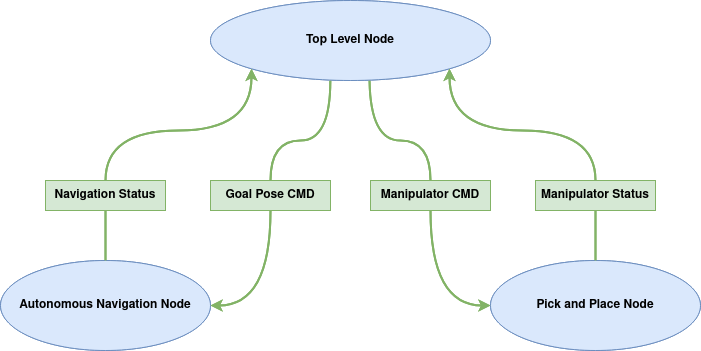
\includegraphics[width = 0.9\textwidth]{Figures/figTopLevelMethod.drawio.png}
    \caption{This figure illustrates on a high level how the main systems in the solution interacts with each other to orchestrate a warehouse automation task. The Top Level Node commands and receives feedback from Autonomous Navigation and Pick and Place}
    \label{fig:M:CD:topLevelMethod}
\end{figure}

The top level system should take commands for what object to pick and where this object is located in the warehouse. It should then give commands to both the autonomous navigating system and the pick and place system in order to orchestrate a warehouse automation task. During this operation, this system will need to get feedback on the status of the other systems to decide what to do next.

The autonomous navigation system should be able to take goal poses consisting of $x,y,\theta$ coordinates, from the top level algorithm. It should then plan it's trajectory, using either Djikstra's algorithm or A*, and autonomously navigate towards the goal pose without the assistance of any operator. During this operation, a SLAM algorithm should be running to provide an updated map of the robot's environment as well as robust localisation. It should also have a collision avoidance system capable of detecting and avoiding collision with moving objects such as workers in the warehouse. When the mobile robot has reached it's goal, the system should report back to the top level system that the goal has been reached.

The pick and place system should consist of a manipulator and a machine vision system that will be a part of the mobile robot. The system should be able to take commands from the top level system and act accordingly. Example of commands are "pick", "place" and "sleep". During picking, machine vision should be utilised for object detection and pose estimation. The system should give feedback on it's current status to the top level system.





The design of the mobile robot should reflect the intended warehouse automation task. This places some requirements on the design that needs to be considered when setting up the robotic system. The requirements gives design specification where a few major components are needed:

\begin{itemize}
    \item A mobile robotic platform capable of housing a robotic manipulator.
    \item A manipulator that supports mounting on mobile robotic platforms.
    \item Sensors to prepare the mobile robot for autonomous navigation
    \item Sensors to prepare the manipulator for machine vision based object detection and pose estimation.
\end{itemize}

\subsection{Initial Concept} \label{sec:M:CD:InitialConcept}
With the described design specifications considered, the initial conceptual design resulted in the following major components:

\begin{itemize}
    \item Clearpath - Husky A200 UGV
    \item Redshift Labs - UM7 IMU
    \item Ouster -  OS1-64 3D LiDAR
    \item Universal Robots - UR5
    \item Intel - Realsense D435i Camera
    \item 2 X NVIDIA - Jetson AGX Xavier
\end{itemize}

From the bulletin list above, Husky A200, seen in figure \ref{fig:huskyA200}, provides a robust mobile platform and UM7 IMU and Ouster OS1-64 LiDAR provides sensory information to allow for autonomous navigation. The UR5 robotic manipulator, seen in figure \ref{fig:ur5}, paired with an Intel Realsense D435i, adds capabilities for pick and place operations with object detection and 6-DOF pose estimation. The two NVIDIA Jetson AGX Xaviers will be used to control the platform.

\begin{figure}[H]
  \centering
  \begin{minipage}[b]{0.49\textwidth}
        \centering
        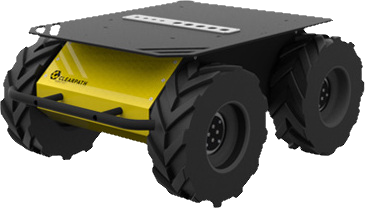
\includegraphics[width = 0.8\textwidth]{Figures/huskyA200.png}
        \caption{Clearpath Husky A200. Image adapted from \cite{clearpath_husky_website}}
        \label{fig:huskyA200}
  \end{minipage}
  \hfill
  \begin{minipage}[b]{0.49\textwidth}
    \centering
    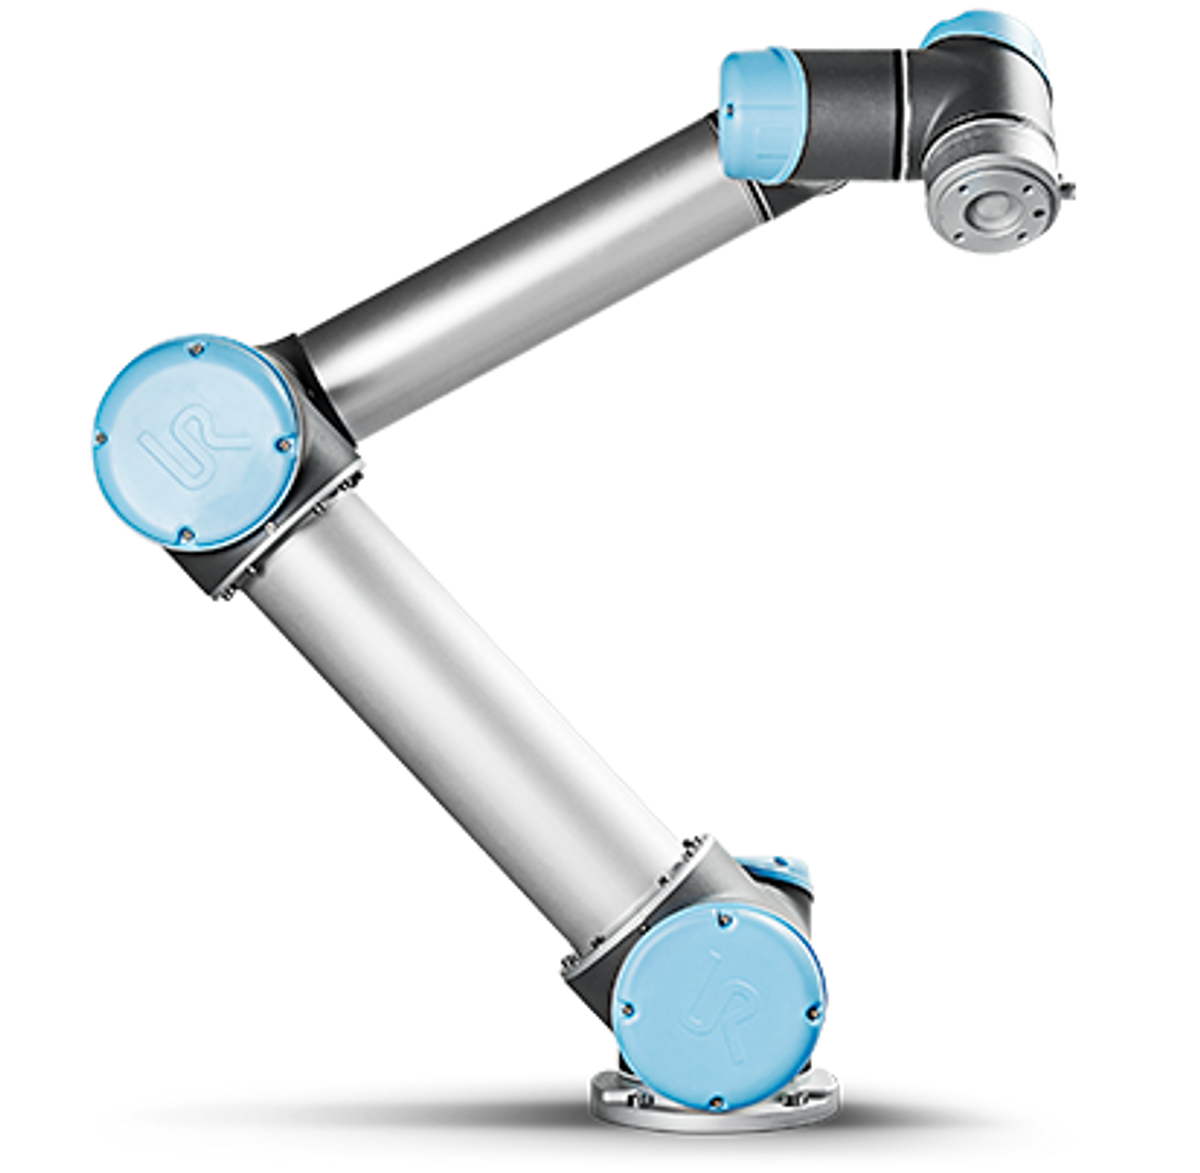
\includegraphics[width = 0.8\textwidth]{Figures/ur5.png}
    \caption{Universal Robots UR5. Image from \cite{ur5_img}}
    \label{fig:ur5}
  \end{minipage}
\end{figure}

Some specifications on the Husky A200 robotic platform is listed in table \ref{tab:husky:a200:specs}

\begin{table}[H]
\centering
\caption{Technical specifications for the Clearpath Husky A200, complete data sheet available in appendix \ref{A:fig:husky_data_sheet}, from \cite{clearpath_husky_website}}
\label{tab:husky:a200:specs}
\vspace{1mm}
\begin{tabular}{ll}
\hline
\multicolumn{2}{c}{\textbf{Husky A200 Specifications}}                                                            \\ \hline
Drivers and APIs                            & ROS, ROS 2, C++ and Python                                          \\
Wheel encoders                              & Quadrature: 78,000 {[}pulses/m{]}
        \\
Communication                               & RS232@115200 Baud                                                   \\
Battery                                     & \begin{tabular}[c]{@{}l@{}}12V 20Ah\\ Sealed Lead Acid\end{tabular} \\
\multicolumn{1}{c}{User Power Distribution} & \begin{tabular}[c]{@{}l@{}}5V 5A\\  12V 5A\\  24V 5A\end{tabular}   \\
Weight                                      & 50 {[}kg{]}                                                         \\
Payload Capacity                            & 75 {[}kg{]}                                                         \\
External Dimensions                         & 990 x 670 x 390 {[}mm{]}                                            \\ \hline
\end{tabular}
\end{table}

One NVIDIA Jetson AGX Xavier, hereby called "UGV Xavier", interfaces with Husky, LiDAR and IMU. This computer will control the Husky and take care of autonomous navigation tasks such as mapping, localization and path planning. 

The second NVIDIA Jetson AGX Xavier, hereby called Manipulator Xavier, interfaces with the Realsense camera and robotic manipulator. This computer will control the manipulator, and take care of sensory information from the Realsense camera. 

The relatively powerful GPU of the Xaviers adds capabilities to implement deep learning algorithms to do for example image- or PointCloud based object detection.

\subsection{Final Concept}\label{sec:M:CD:FinalConcept}

The UR5 manipulator requires a dedicated controller to operate.This controller also contains the DC-power supply for the manipulator. As the manipulator is to be mounted on an UGV, this controller has to be powered through DC-power. According to the Universal Robots CB3 battery supply installation manual \cite{ur5_battery_manual}, the UR5 could draw up to 50A at "peak conditions". Looking at table \ref{tab:husky:a200:specs}, it is clear that the built in 24V power distribution on the Husky, with a 5A circuit breaker, is insufficient.

The design of a mobile power system for the CB3 controller and thus, the UR5 manipulator is beyond the scope of this project. The decision was therefore made to swap out the UR5 manipulator with a smaller Interbotix VX300 manipulator from Trossen Robotics, illustrated in figure \ref{fig:M:CD:FC:VX300}. This is a significantly smaller robotic arm that is powered through 12V DC-power supply with a standard 2.5mm DC barrel jack. Some of it's key specifications is shown in table \ref{tab:M:CD:FC:VX300Specs}

\begin{figure}[H]
    \centering
    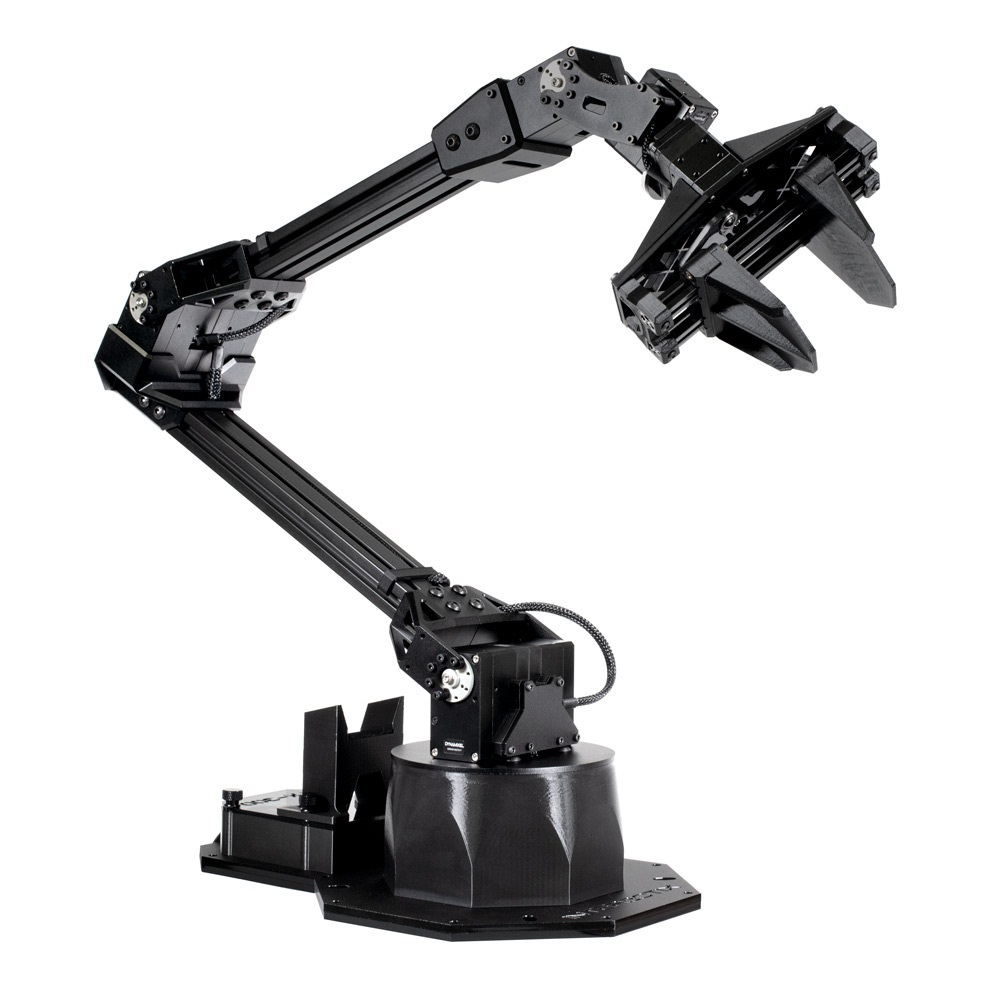
\includegraphics[width = 0.5\textwidth]{Figures/VX300.jpg}
    \caption{Interbotix VX300. Image from \cite{interbotix_vx300}}
    \label{fig:M:CD:FC:VX300}
\end{figure}

\begin{table}[H]
\centering
\caption{Technical Specifications for the Interbotix VX300 Manipulator. From \cite{interbotix_vx300}}
\label{tab:M:CD:FC:VX300Specs}
\vspace{1mm}
\begin{tabular}{ll}
\hline
\multicolumn{2}{c}{\textbf{Interbotix VX300 Specifications}} \\ \hline
Degrees of Freedom               & 5                         \\
Reach                            & 750{[}mm{]}               \\
Span                             & 1500{[}mm{]}              \\
Accuracy                         & 5-8{[}mm{]}               \\
Working Payload                  & 750{[}g{]}                \\ \hline
\end{tabular}
\end{table}


  
\section{Hardware}\label{sec:H:Hardware}
This section describes the different hardware components of the robotic system and how they are set up for this project. A high level overview of the network topology is shown in figure \ref{fig:topology}. This topology gives an insight to how the different components are connected to create a complete system. Looking at figure \ref{fig:topology}, it can be seen that the UGV Xavier communicates with the Husky through RS232 and the UM7 IMU through USB. The LiDAR communicates through Ethernet via a WiFi router that, in this case acts as a switch. The LiDAR data is therefore available for all computers on the network. From figure \ref{fig:topology}, it can be seen that the Manipulator Xavier interfaces with both the Realsense camera and the manipulator through USB. 

\begin{figure}[H]
  \centering
  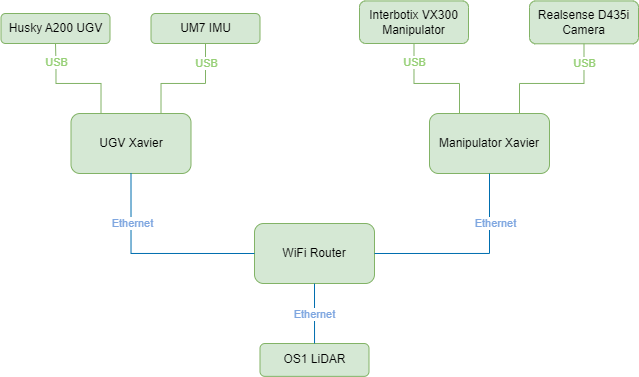
\includegraphics[width = 0.9\textwidth]{Figures/example_figure.drawio.png}
  \caption{High level network topology showing the various components on the mobile robotic platform}
  \label{fig:topology}
\end{figure}

The WiFi Router allows external computers to connect to the network, either through WiFi or cabled connection, and communicate with the two Xaviers and the LiDAR. This makes it possible to control the Xavier computers through SSH and also allows developers to interact with the ROS2 network.

\subsection{General Arrangement}\label{M:H:GeneralArrangement}
By comparing figure \ref{fig:M:H:CHS:CadHuskyComplete} and figure \ref{fig:M:H:CHS:PhysHuskyComplete}, it can be seen that there are a few more auxiliary components attached to the experimental system. A general arrangement drawing describing the physical arrangement of all the components mounted on the UGV is presented in figure \ref{fig:general_arrangement}.

\begin{figure}[H]
  \centering
   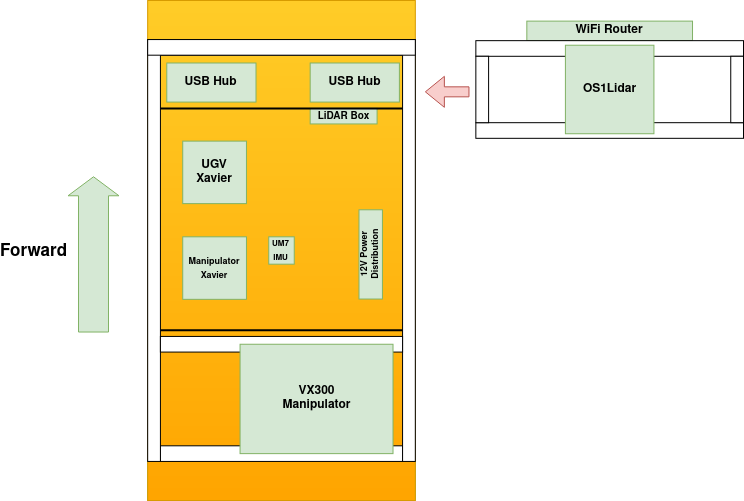
\includegraphics[width = 0.9\textwidth]{Figures/general_arrangement.drawio.png}
  \caption{General arrangement drawing of UGV platform. Here, the physical position of different hardware components are defined. The sensor frame is drawn to the left of the main frame.}
  \label{fig:general_arrangement}
\end{figure}

\subsection{Electrical Interface}\label{M:H:ElectricalInterface}
The different components in the system is powered through the user power supply of the UGV(see table \ref{tab:husky:a200:specs}). Figure \ref{fig:circuit_diagram} is a circuit diagram that illustrates the DC power distribution.

\begin{figure}[H]
  \centering
  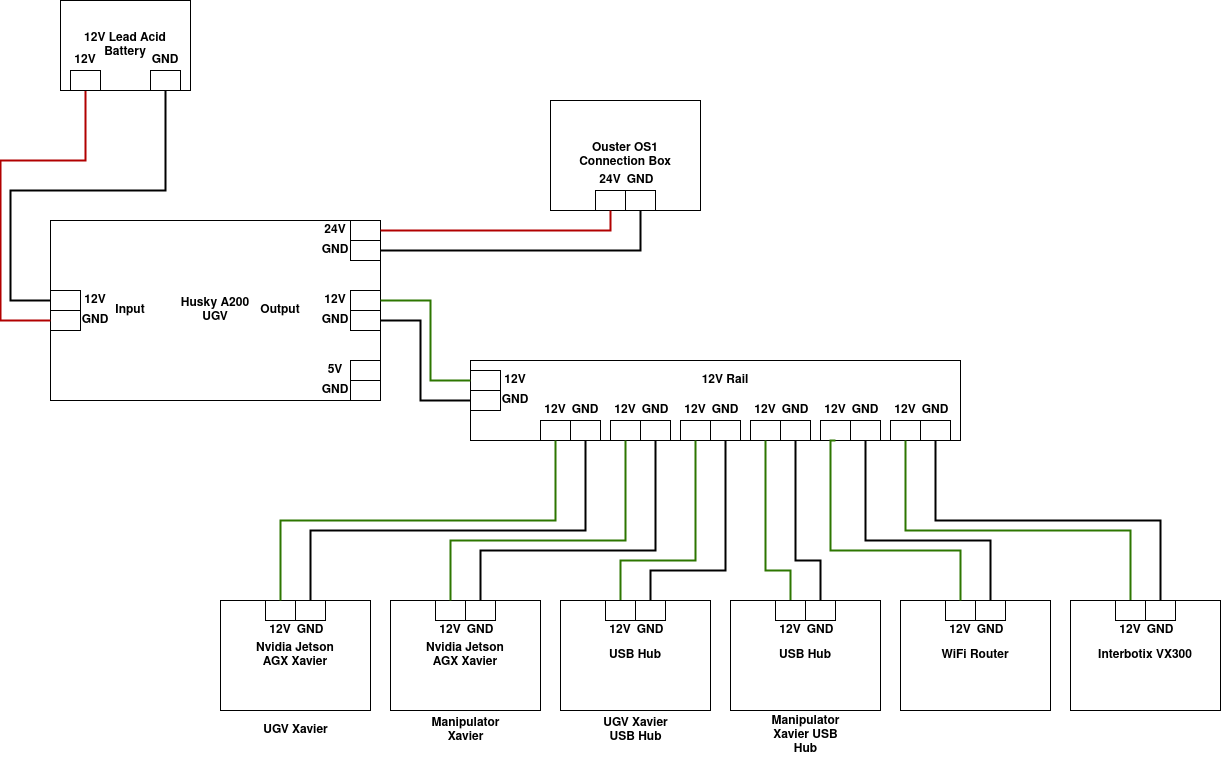
\includegraphics[width = 1\textwidth]{Figures/circuit_diagram.drawio.png}
  \caption{Circuit diagram showing the power distribution on the UGV}
  \label{fig:circuit_diagram}
\end{figure}

\subsection{Autonomous Navigation Hardware}\label{sec:M:H:Autonomous Navigation Hardware}

\subsubsection{Accessory mounting frame}\label{sec:M:H:AccessoryMountingFrame}
As the UGV is to be used for prototyping and testing, it is preferable to have some kind of bracket where various sensors and actuators could be mounted. The bracket should be rigid, yet flexible in terms of mounting possibilities. An aluminium profile frame is therefore designed for the UGV.

The aluminium frame, seen in figure \ref{fig:M:H:AMF:userFrame} is made out of 20X20mm aluminium profiles. The purpose of the frame is to add the possibility to mount whatever accessory the developer wants to the UGV. The choice fell on 20X20mm aluminium profiles as they are practical for mounting various equipment as well as the fact that the Husky A200 UGV is delivered with a 20x20mm mounting frame out of the box. Looking at figure \ref{fig:M:H:AMF:userFrame}, the husky mounting frame can be seen as the rectangular black frame on top of the Husky UGV.

\begin{figure}[H]
  \centering
  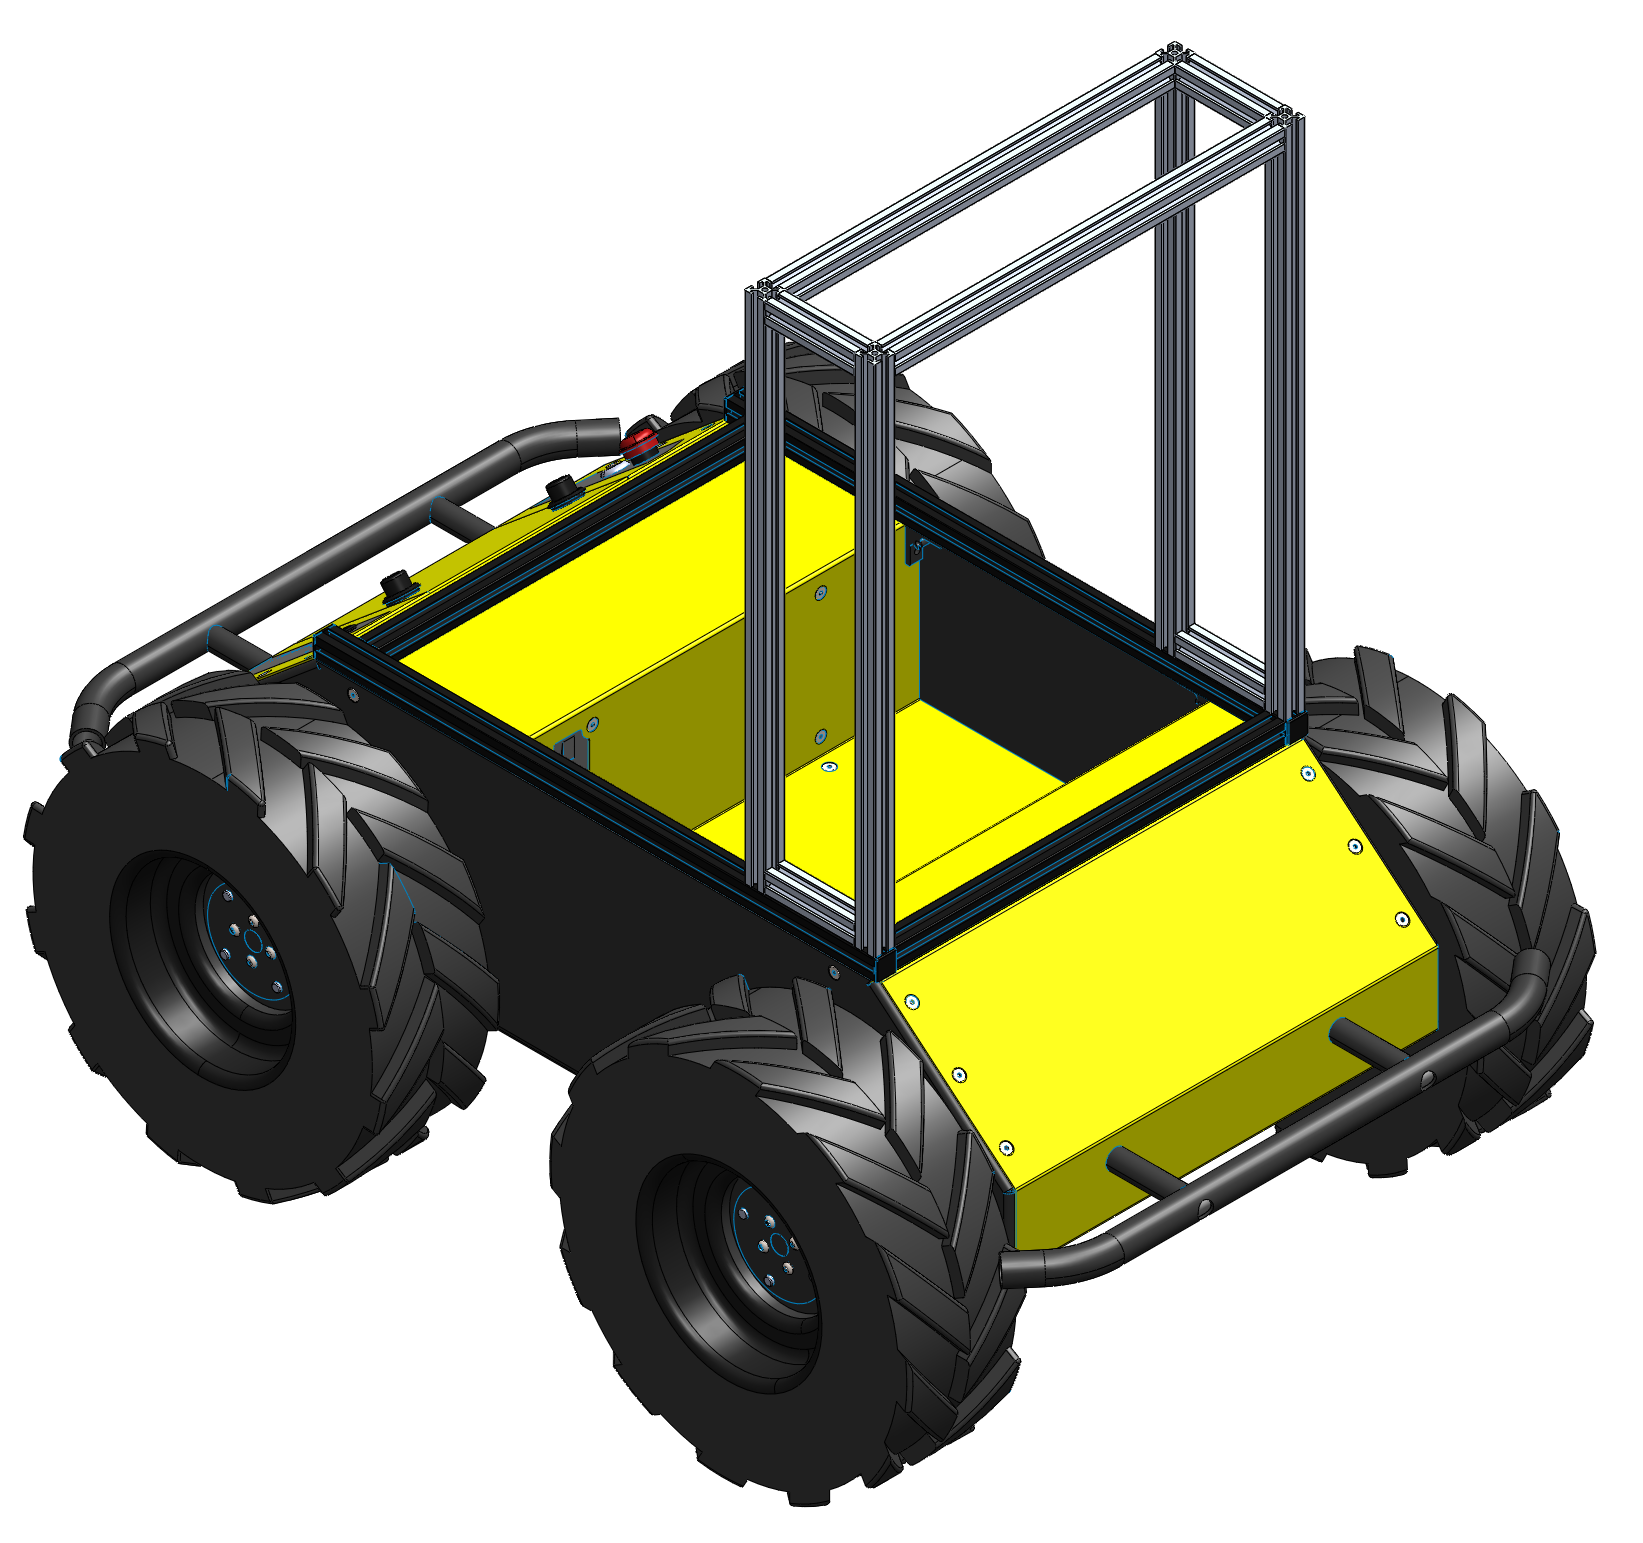
\includegraphics[width = 0.7\textwidth]{Figures/husky_with_frame.png}
  \caption{CAD model of Husky A200 with sensor frame mounted}
  \label{fig:M:H:AMF:userFrame}
\end{figure}

\subsubsection{IMU}\label{sec:M:H:ANH:IMU}
In order to increase the performance of the UGV odometry, an UM7 IMU from Redshift Labs, seen in figure \ref{fig:um7_imu}, has been added. This IMU is ROS2 compatible and will publish IMU data to ROS2. This data can then be used to better calculate the position of the UGV. 

\begin{figure}[H]
  \centering
  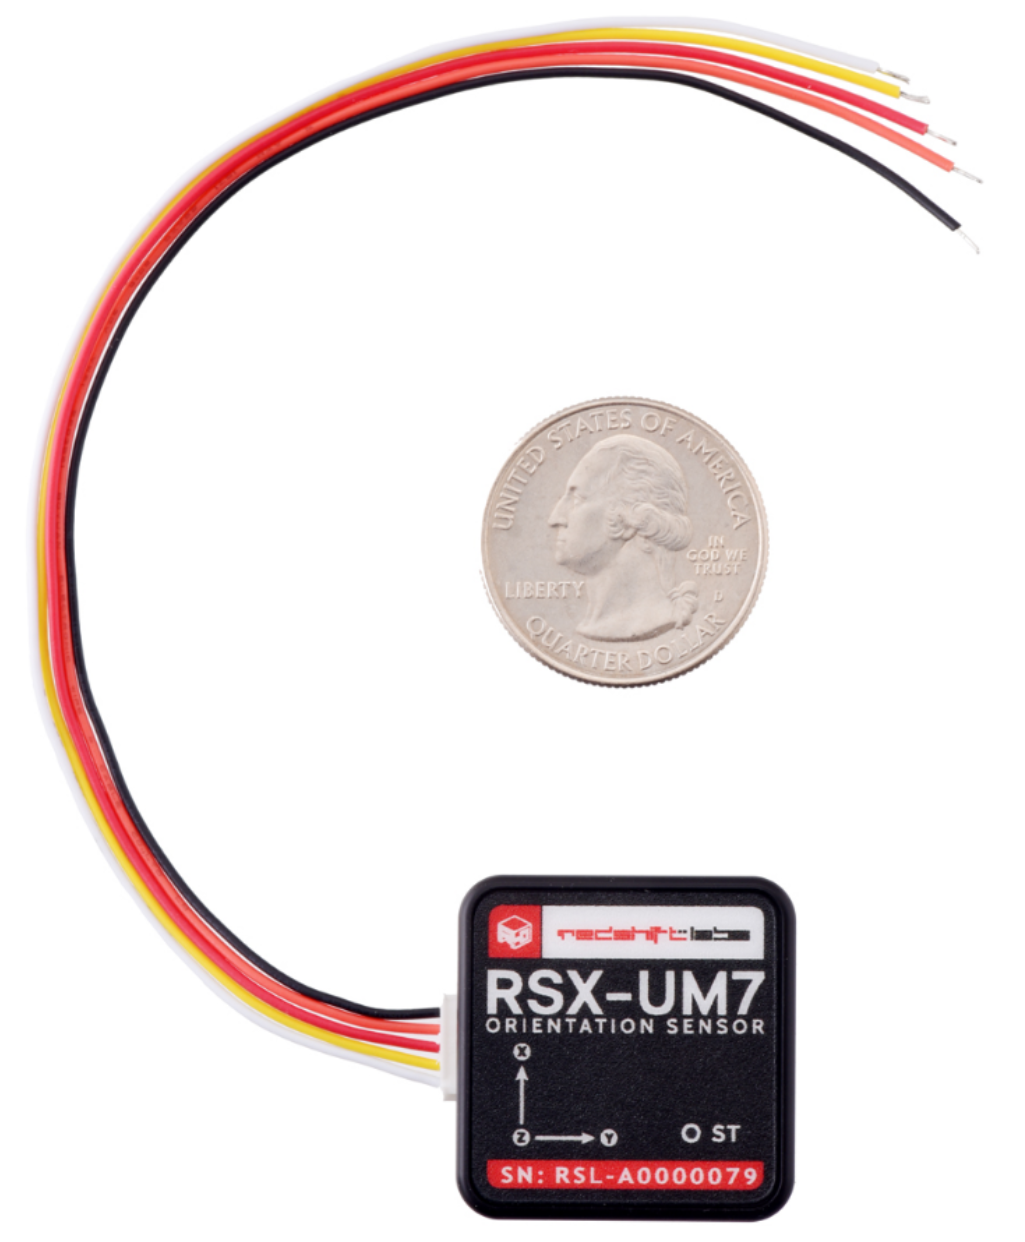
\includegraphics[width = 0.3\textwidth]{Figures/um7_imu.png}
  \caption{Redshift Labs UM7 IMU. Image from \cite{um7_imu}.}
  \label{fig:um7_imu}
\end{figure}

As illustrated in the topology in figure \ref{fig:topology}, the UM7 is connected to the UGV Xavier through USB which is used for power and communication.

\subsubsection{LiDAR}\label{sec:M:H:ANH:Lidar}
The Ouster OS1-64, is a $360\deg$ 3D LiDAR that generates a large amount of spatial information about the surrounding environment as a point cloud. In this project, that point cloud is used for localisation and to generate a 2D map of the environment. The OS1-164 LiDAR is fitted with a built in IMU sensor which for example can be used the same way, or together with, the UM7 IMU for localisation. The LiDAR can be seen mounted on a camera bracket in figure \ref{fig:lidar_mount}.

\subsubsection{LiDAR and Camera Mount}\label{sec:M:H:ANH:LidarAndCameraMount}
To account for the possibility to fuse LiDAR and image data, a LiDAR and camera mount, seen in figure \ref{fig:lidar_mount}, is created. The mount is designed to have the Ouster OS1 LiDAR mounted on the top and four e-con cameras inside. The e-con cameras are arranged $90\deg$ away from each other with a constant radius from the center of the mount.

\begin{figure}[H]
  \centering
  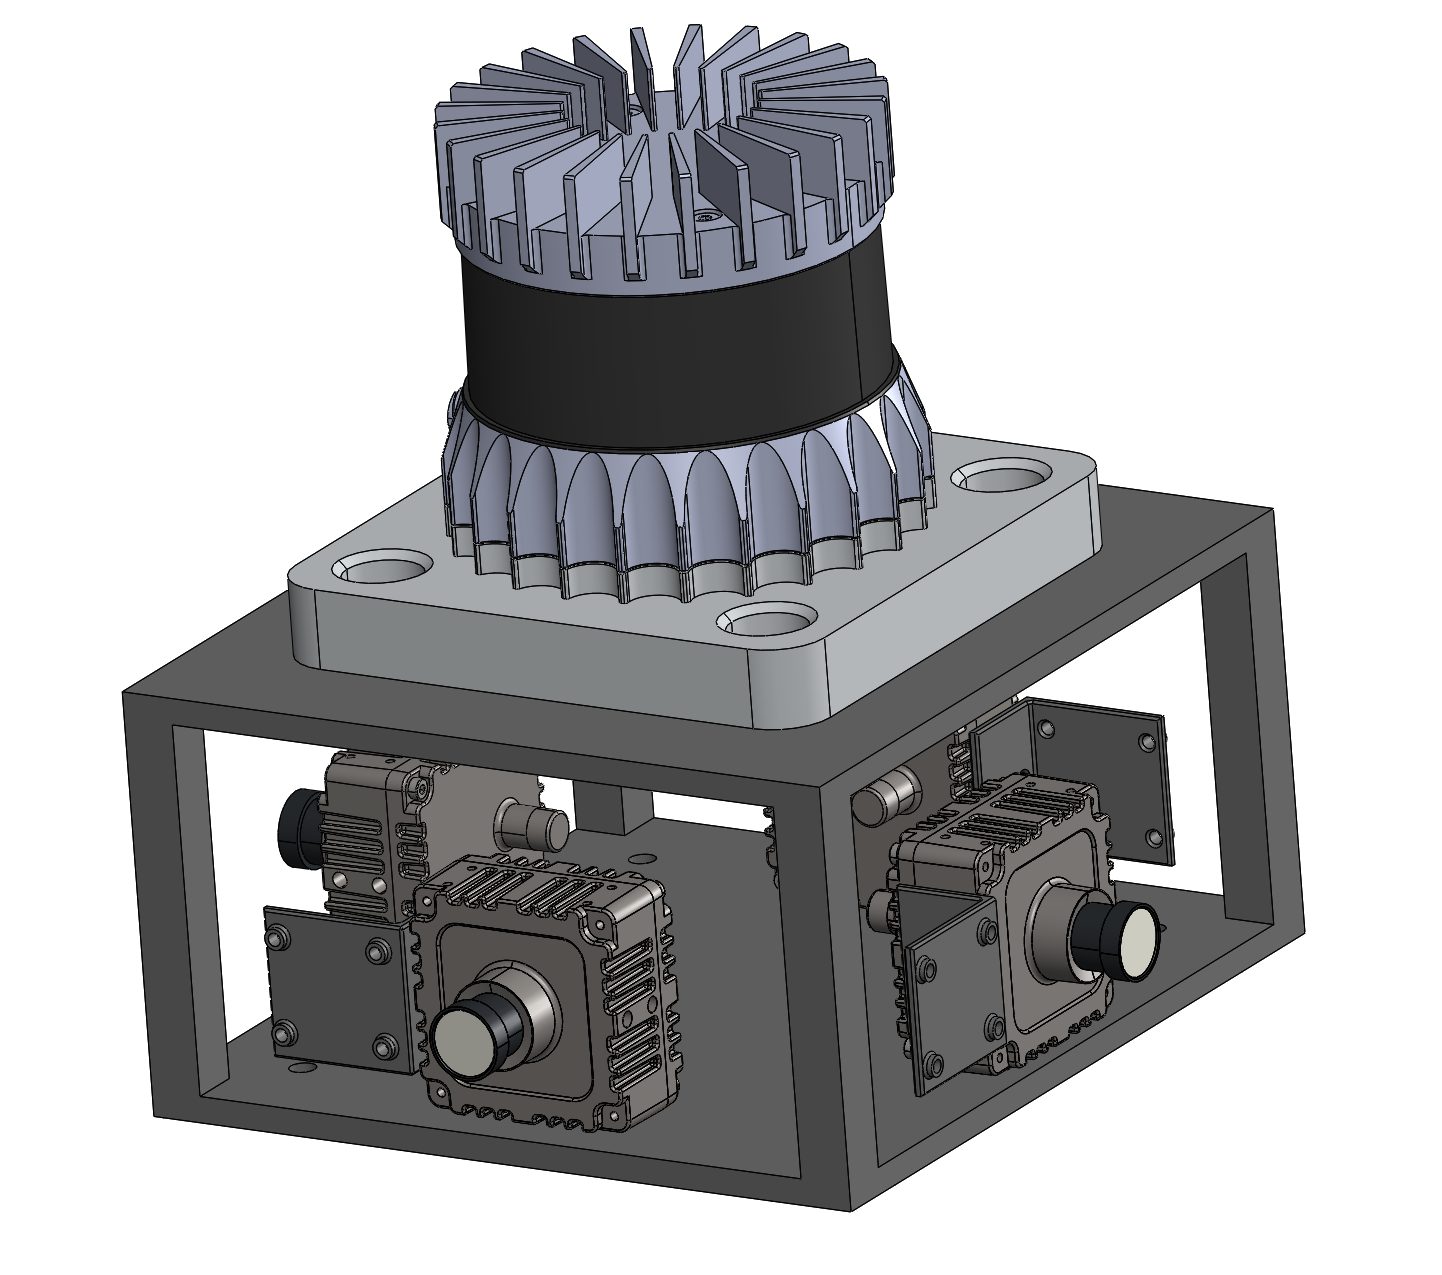
\includegraphics[width = 0.5\textwidth]{Figures/lidar_mount.png}
  \caption{Cad model of LiDAR mount with cameras. The Ouster OS1-64 is mounted on top.}
  \label{fig:lidar_mount}
\end{figure}

\subsection{Pick and Place Hardware}\label{sec:M:H:PickandPlaceHardware}

\subsubsection{Manipulator}\label{sec:M:H:P&PH:Manipulator}
The chosen manipulator, the Interbotix VX300 (figure \ref{fig:M:CD:FC:VX300}, is mounted on the aluminium profiles at the rear right side of the UGV. Offsetting the base of the manipulator from the center of the UGV, gives a longer reach outside of the UGV's footprint. The manipulator requires 12V power through a 2.5mm barrel jack and is connected to the husky user power supply as seen in figure \ref{fig:circuit_diagram}.

\subsubsection{Manipulator Mounted Camera}\label{sec:M:H:P&PH:ManipulatorMountedCamera}
An Intel Realsense D435i camera, seen in figure \ref{fig:d435i}, is mounted on the manipulator to add the possibility of machine vision for pick and place operations. Intel Realsense D435i is a stereo-camera from Intel with 3D vision capabilities and ROS2 compatibility. In order to mount the camera to the manipulator, a bracket has been  designed in CAD software. The bracket is adapted from \cite{d435_sleeve} with modifications to be able to mount it on the gripper of the V300 manipulator. The bracket can be seen in figure \ref{fig:realsense_assembly}.

\begin{figure}[H]
  \centering
  \begin{minipage}[b]{0.49\textwidth}
    \centering
    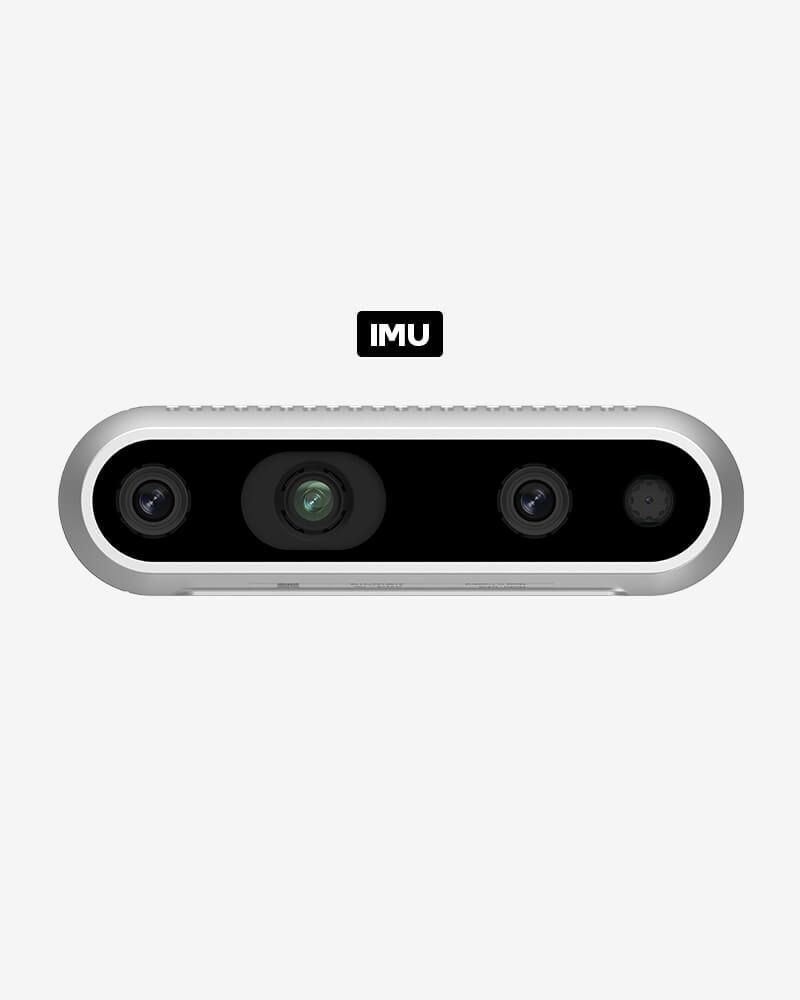
\includegraphics[width = 0.8\textwidth]{Figures/D435i.jpg}
    \caption{Intel Realsense D435i Depth Camera. Image from: \cite{realsense_d435i}.}
    \label{fig:d435i}
  \end{minipage}
  \hfill
  \begin{minipage}[b]{0.49\textwidth}
   \centering
    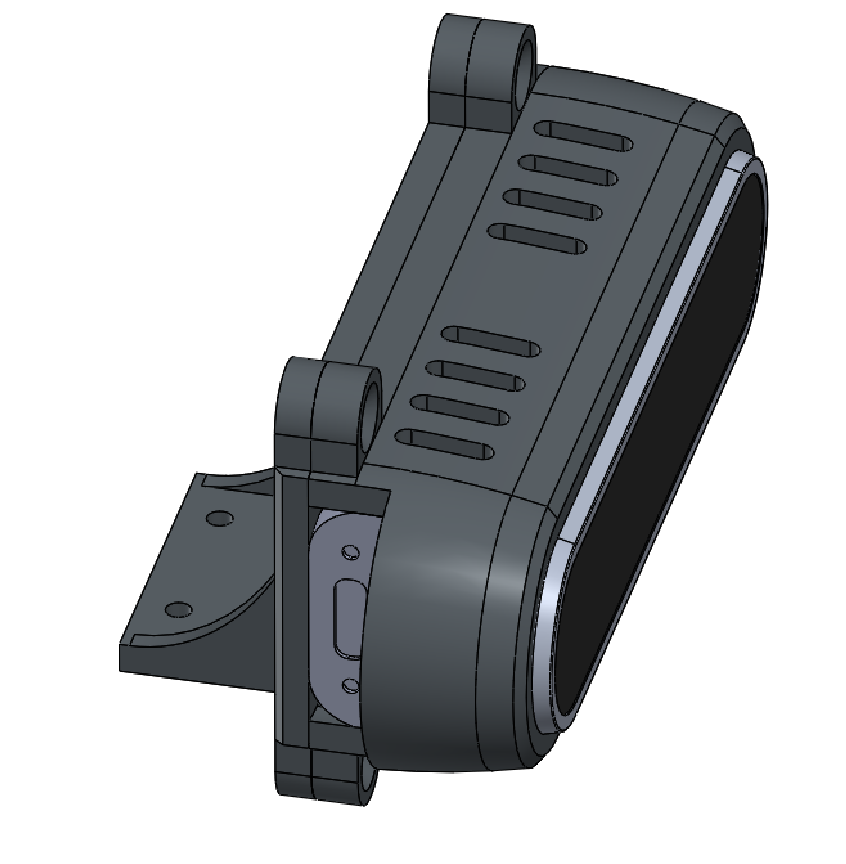
\includegraphics[width = 0.8\textwidth]{Figures/realsense_assembly.pdf}
    \caption{Realsense D435i bracket assembly with camera. The bracket is adapted from \cite{d435_sleeve} to be able to mount on the VX300 robotic arm.}
    \label{fig:realsense_assembly}
  \end{minipage}
\end{figure}

\subsection{Complete Hardware Setup}
The complete hardware setup is presented as a CAD model in figure \ref{fig:M:H:CHS:CadHuskyComplete}. The actual experimental setup is presented in figure \ref{fig:M:H:CHS:PhysHuskyComplete}. 


\begin{figure}[H]
  \centering
  \begin{minipage}[b]{0.49\textwidth}
    \centering
    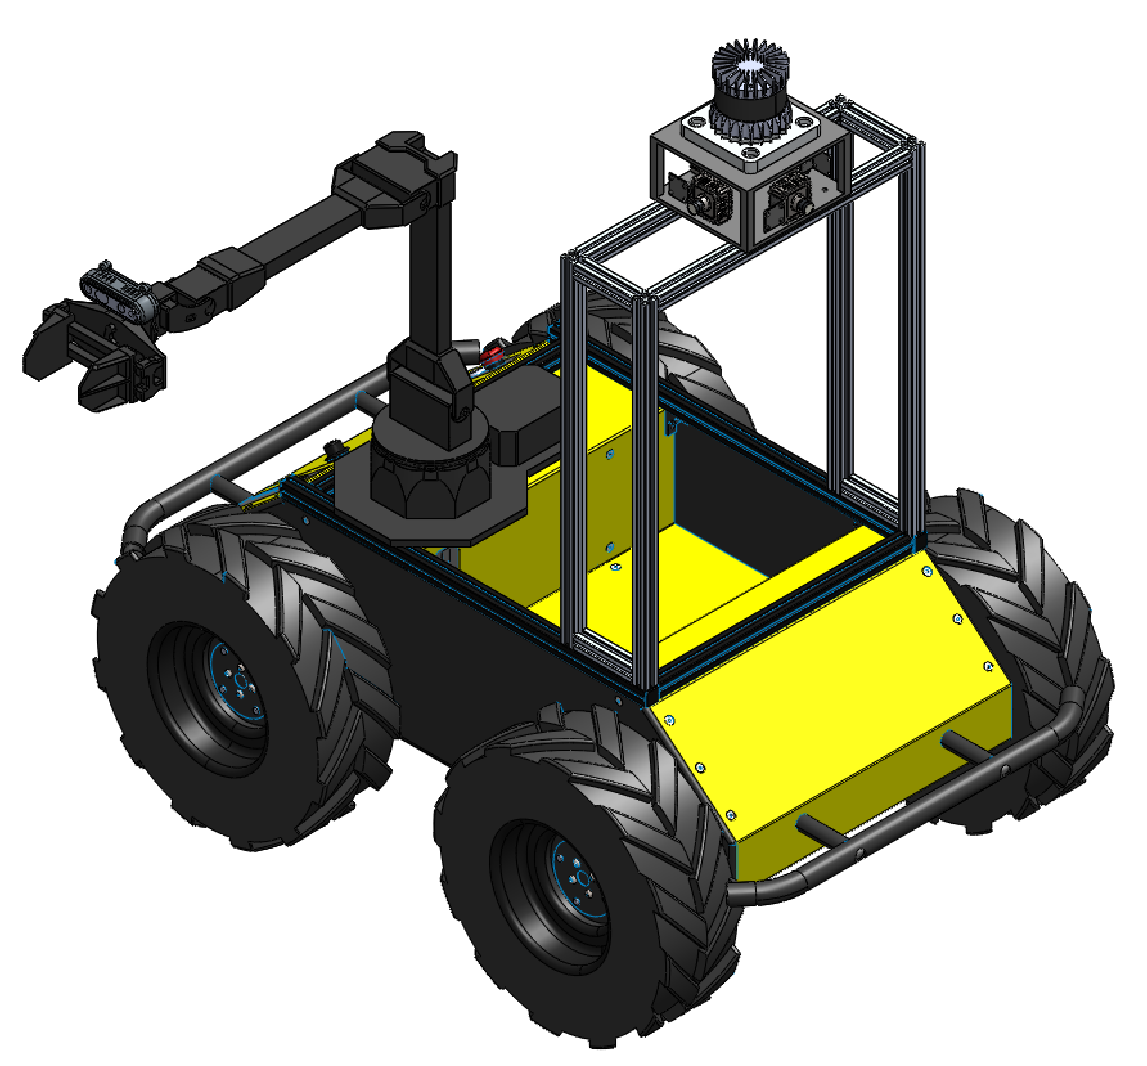
\includegraphics[width = 0.8\textwidth]{Figures/husky_completed.pdf}
    \caption{3D CAD model of the complete robotic system. The accessory mounting frame with the LiDAR mount and the LiDAR is modelled on top of the Husky A200 UGV platform. The VX300 manipulator with it's RealSense D435i camera is mounted at the rear right corner of the UGV platform.}
    \label{fig:M:H:CHS:CadHuskyComplete}
  \end{minipage}
  \hfill
  \begin{minipage}[b]{0.49\textwidth}
    \centering
    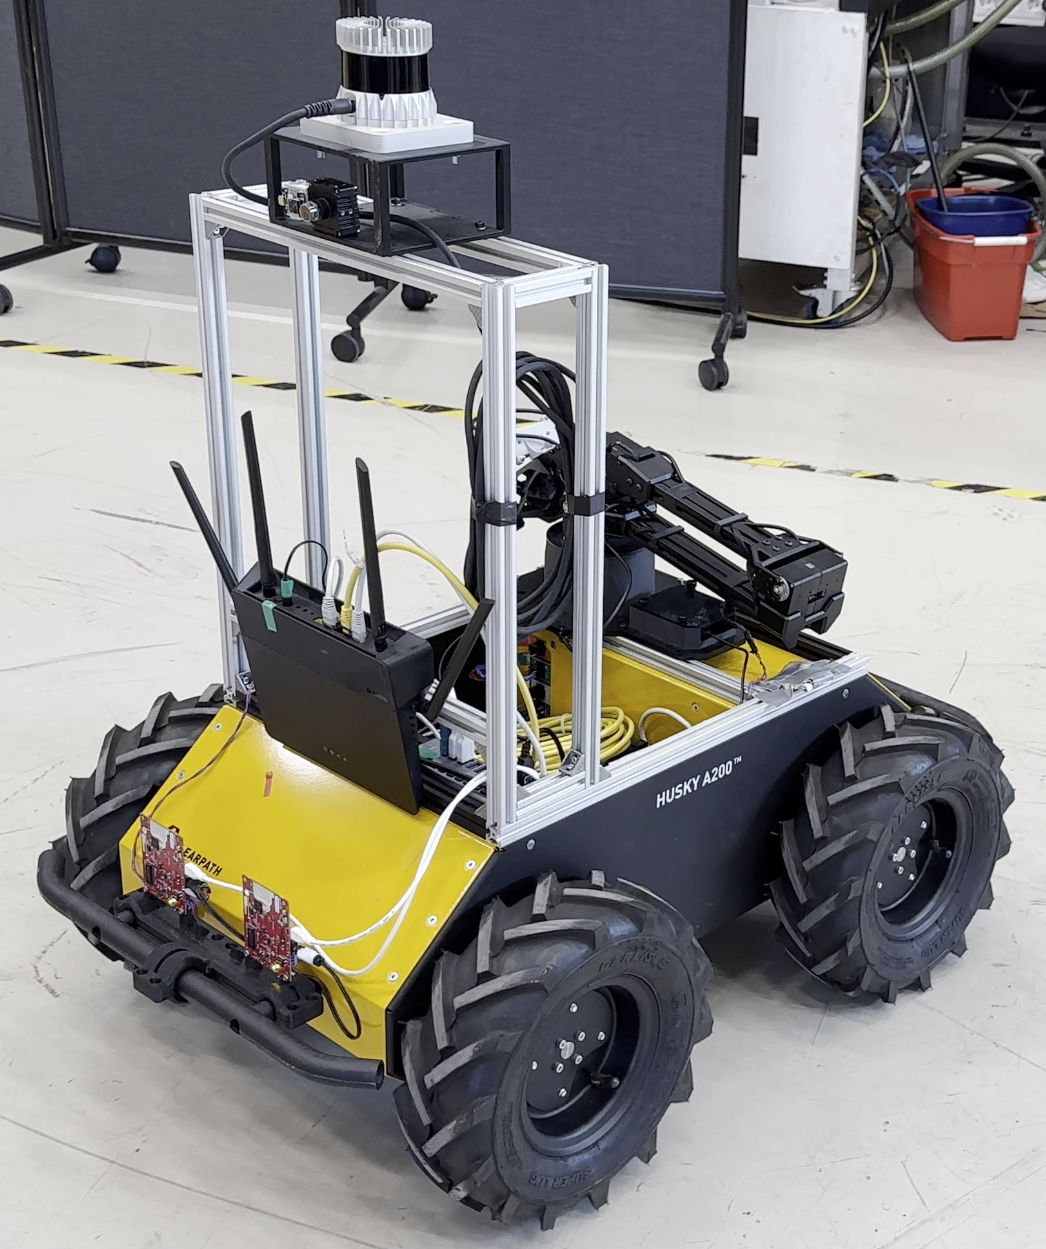
\includegraphics[width = 0.8\textwidth]{Figures/figHuskyComplete.png}
    \caption{Complete experimental robotic system. The accessory mounting frame can be seen mounted on the Husky A200 UGV with the LiDAR mount including the OS1 LiDAR on top. Additionally, it can be seen that the VX300 manipulator is mounted in the rear right corner of the UGV.}
    \label{fig:M:H:CHS:PhysHuskyComplete}
  \end{minipage}
\end{figure}

A closer look at the experimental manipulator setup with it's Realsense D435i bracket and camera is presented in figure \ref{fig:M:H:M:M:MMC:Vx300Complete}.

\begin{figure}[H]
  \centering
  \begin{minipage}[b]{0.49\textwidth}
        \centering
        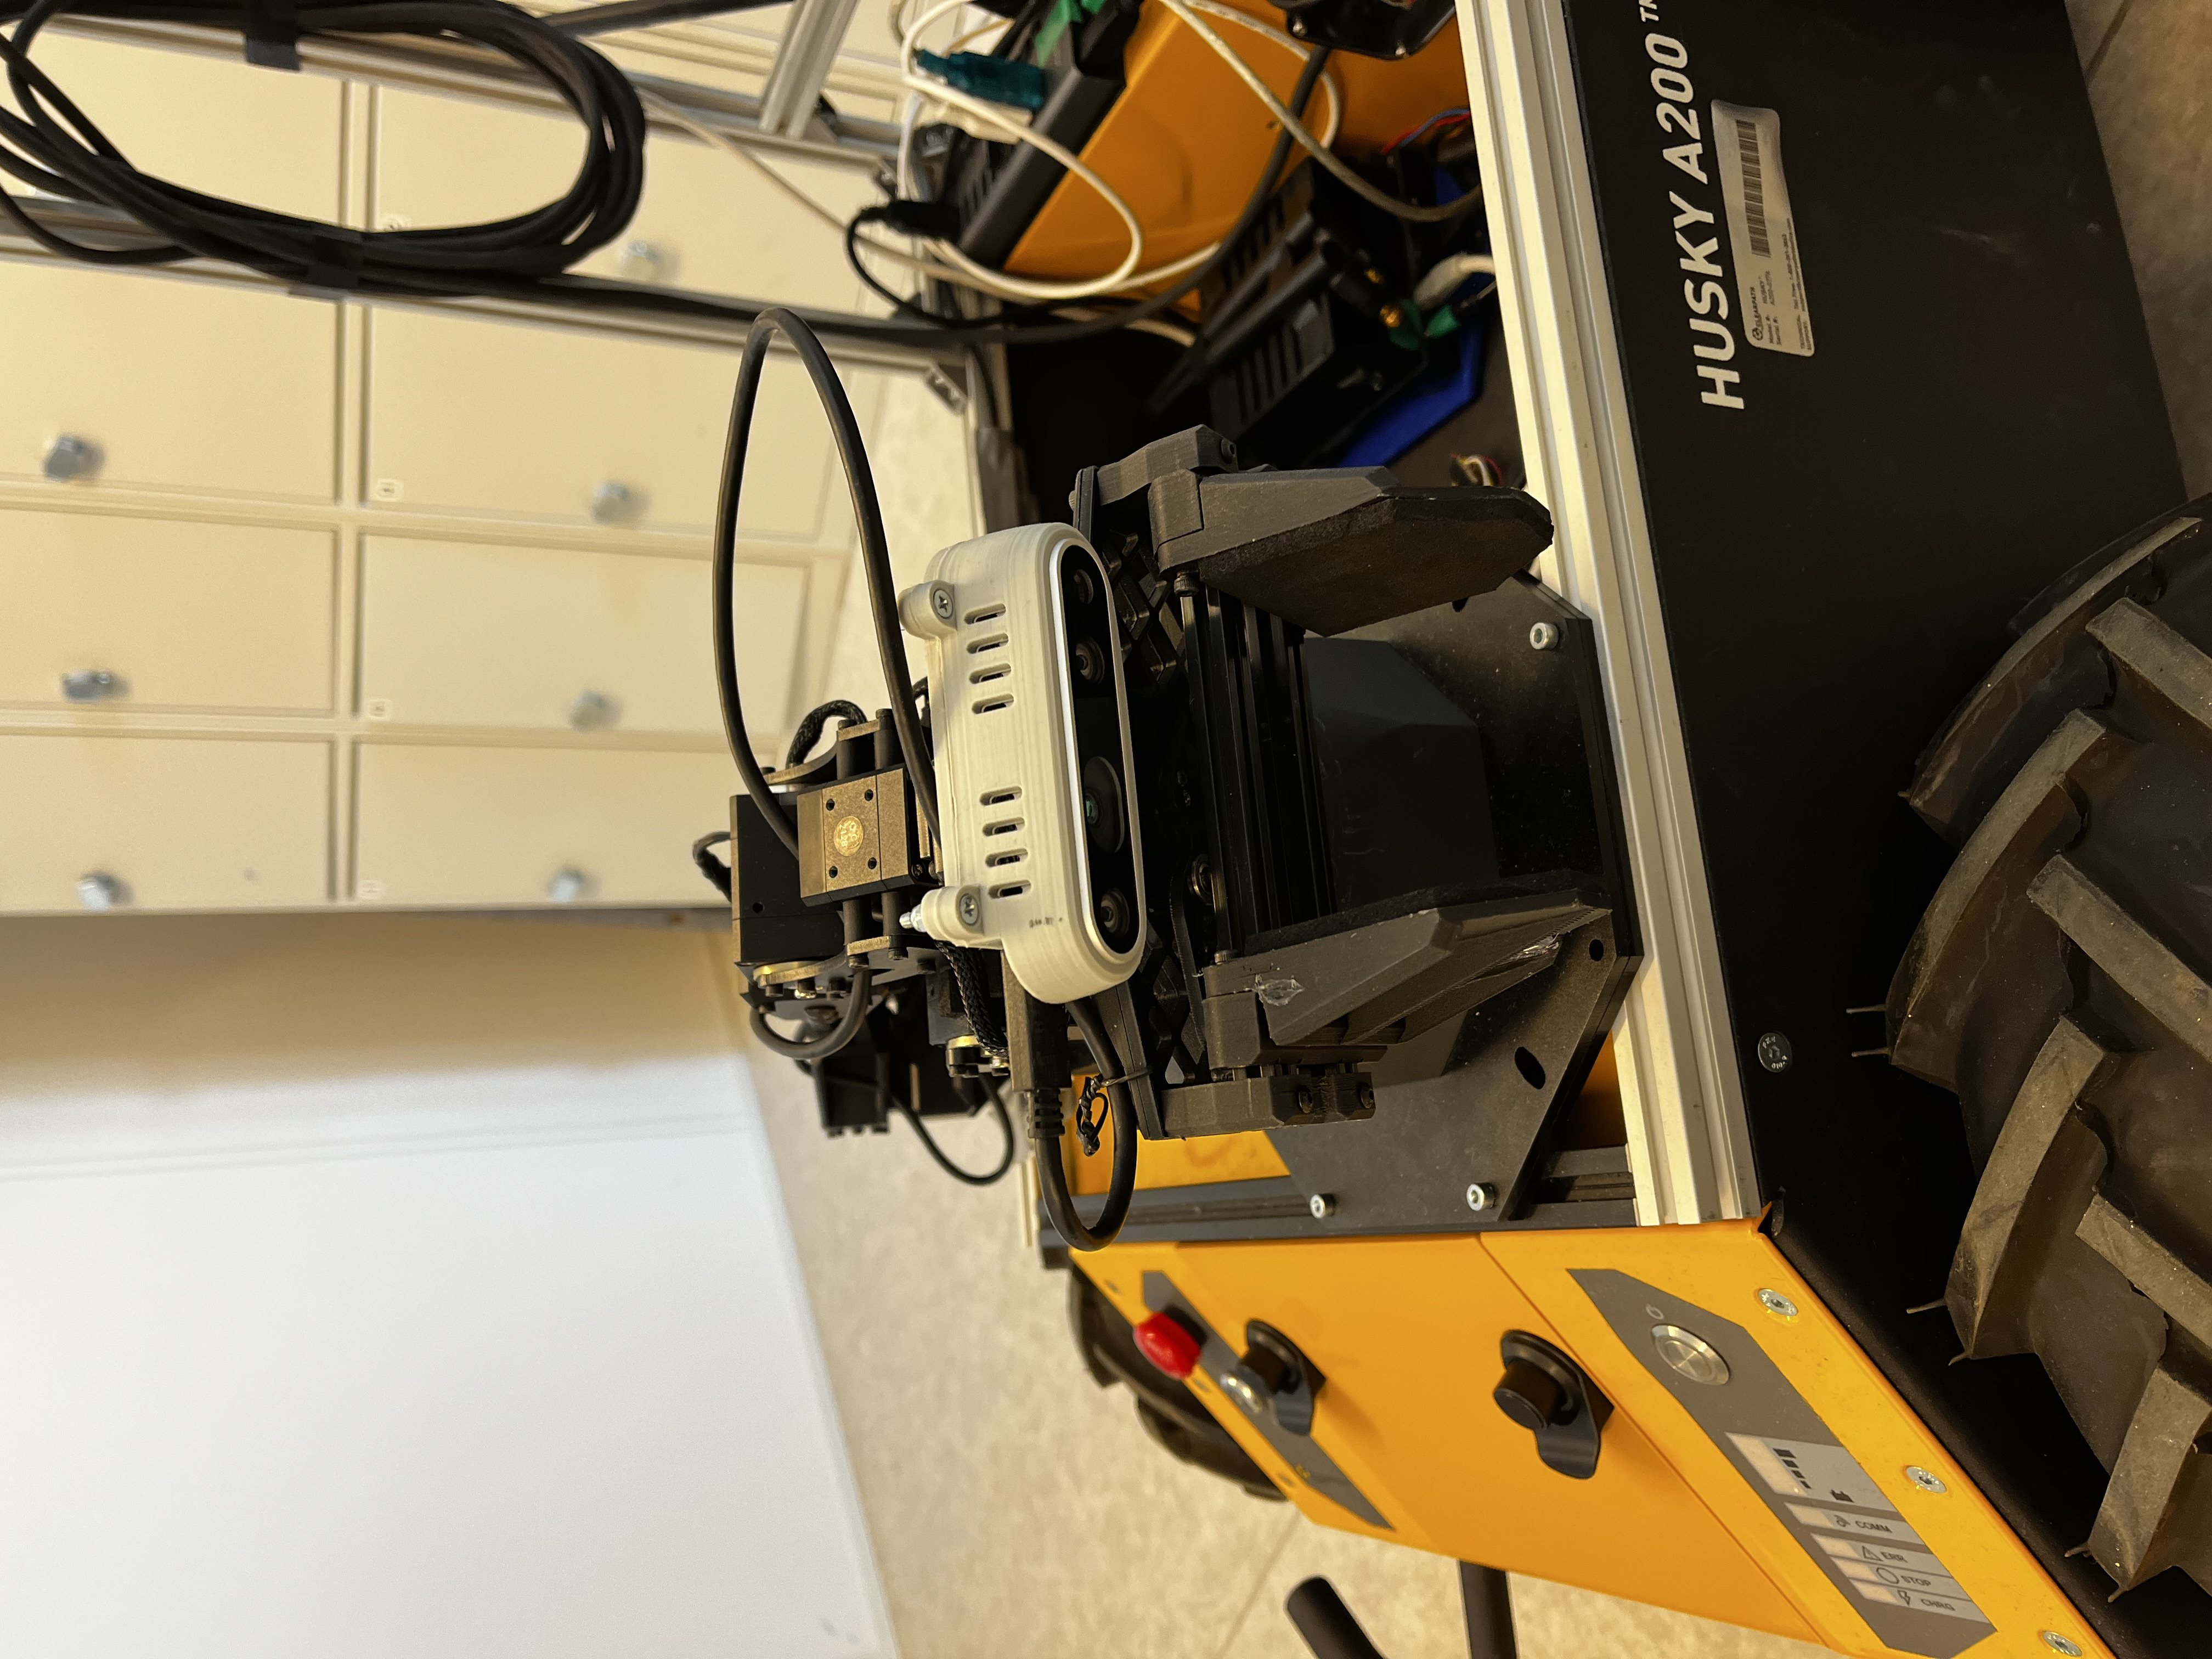
\includegraphics[angle=-90,width = 0.8\textwidth]{Figures/figVX300PhysComplete1.jpg}
  \end{minipage}
  \hfill
  \begin{minipage}[b]{0.49\textwidth}
    \centering
    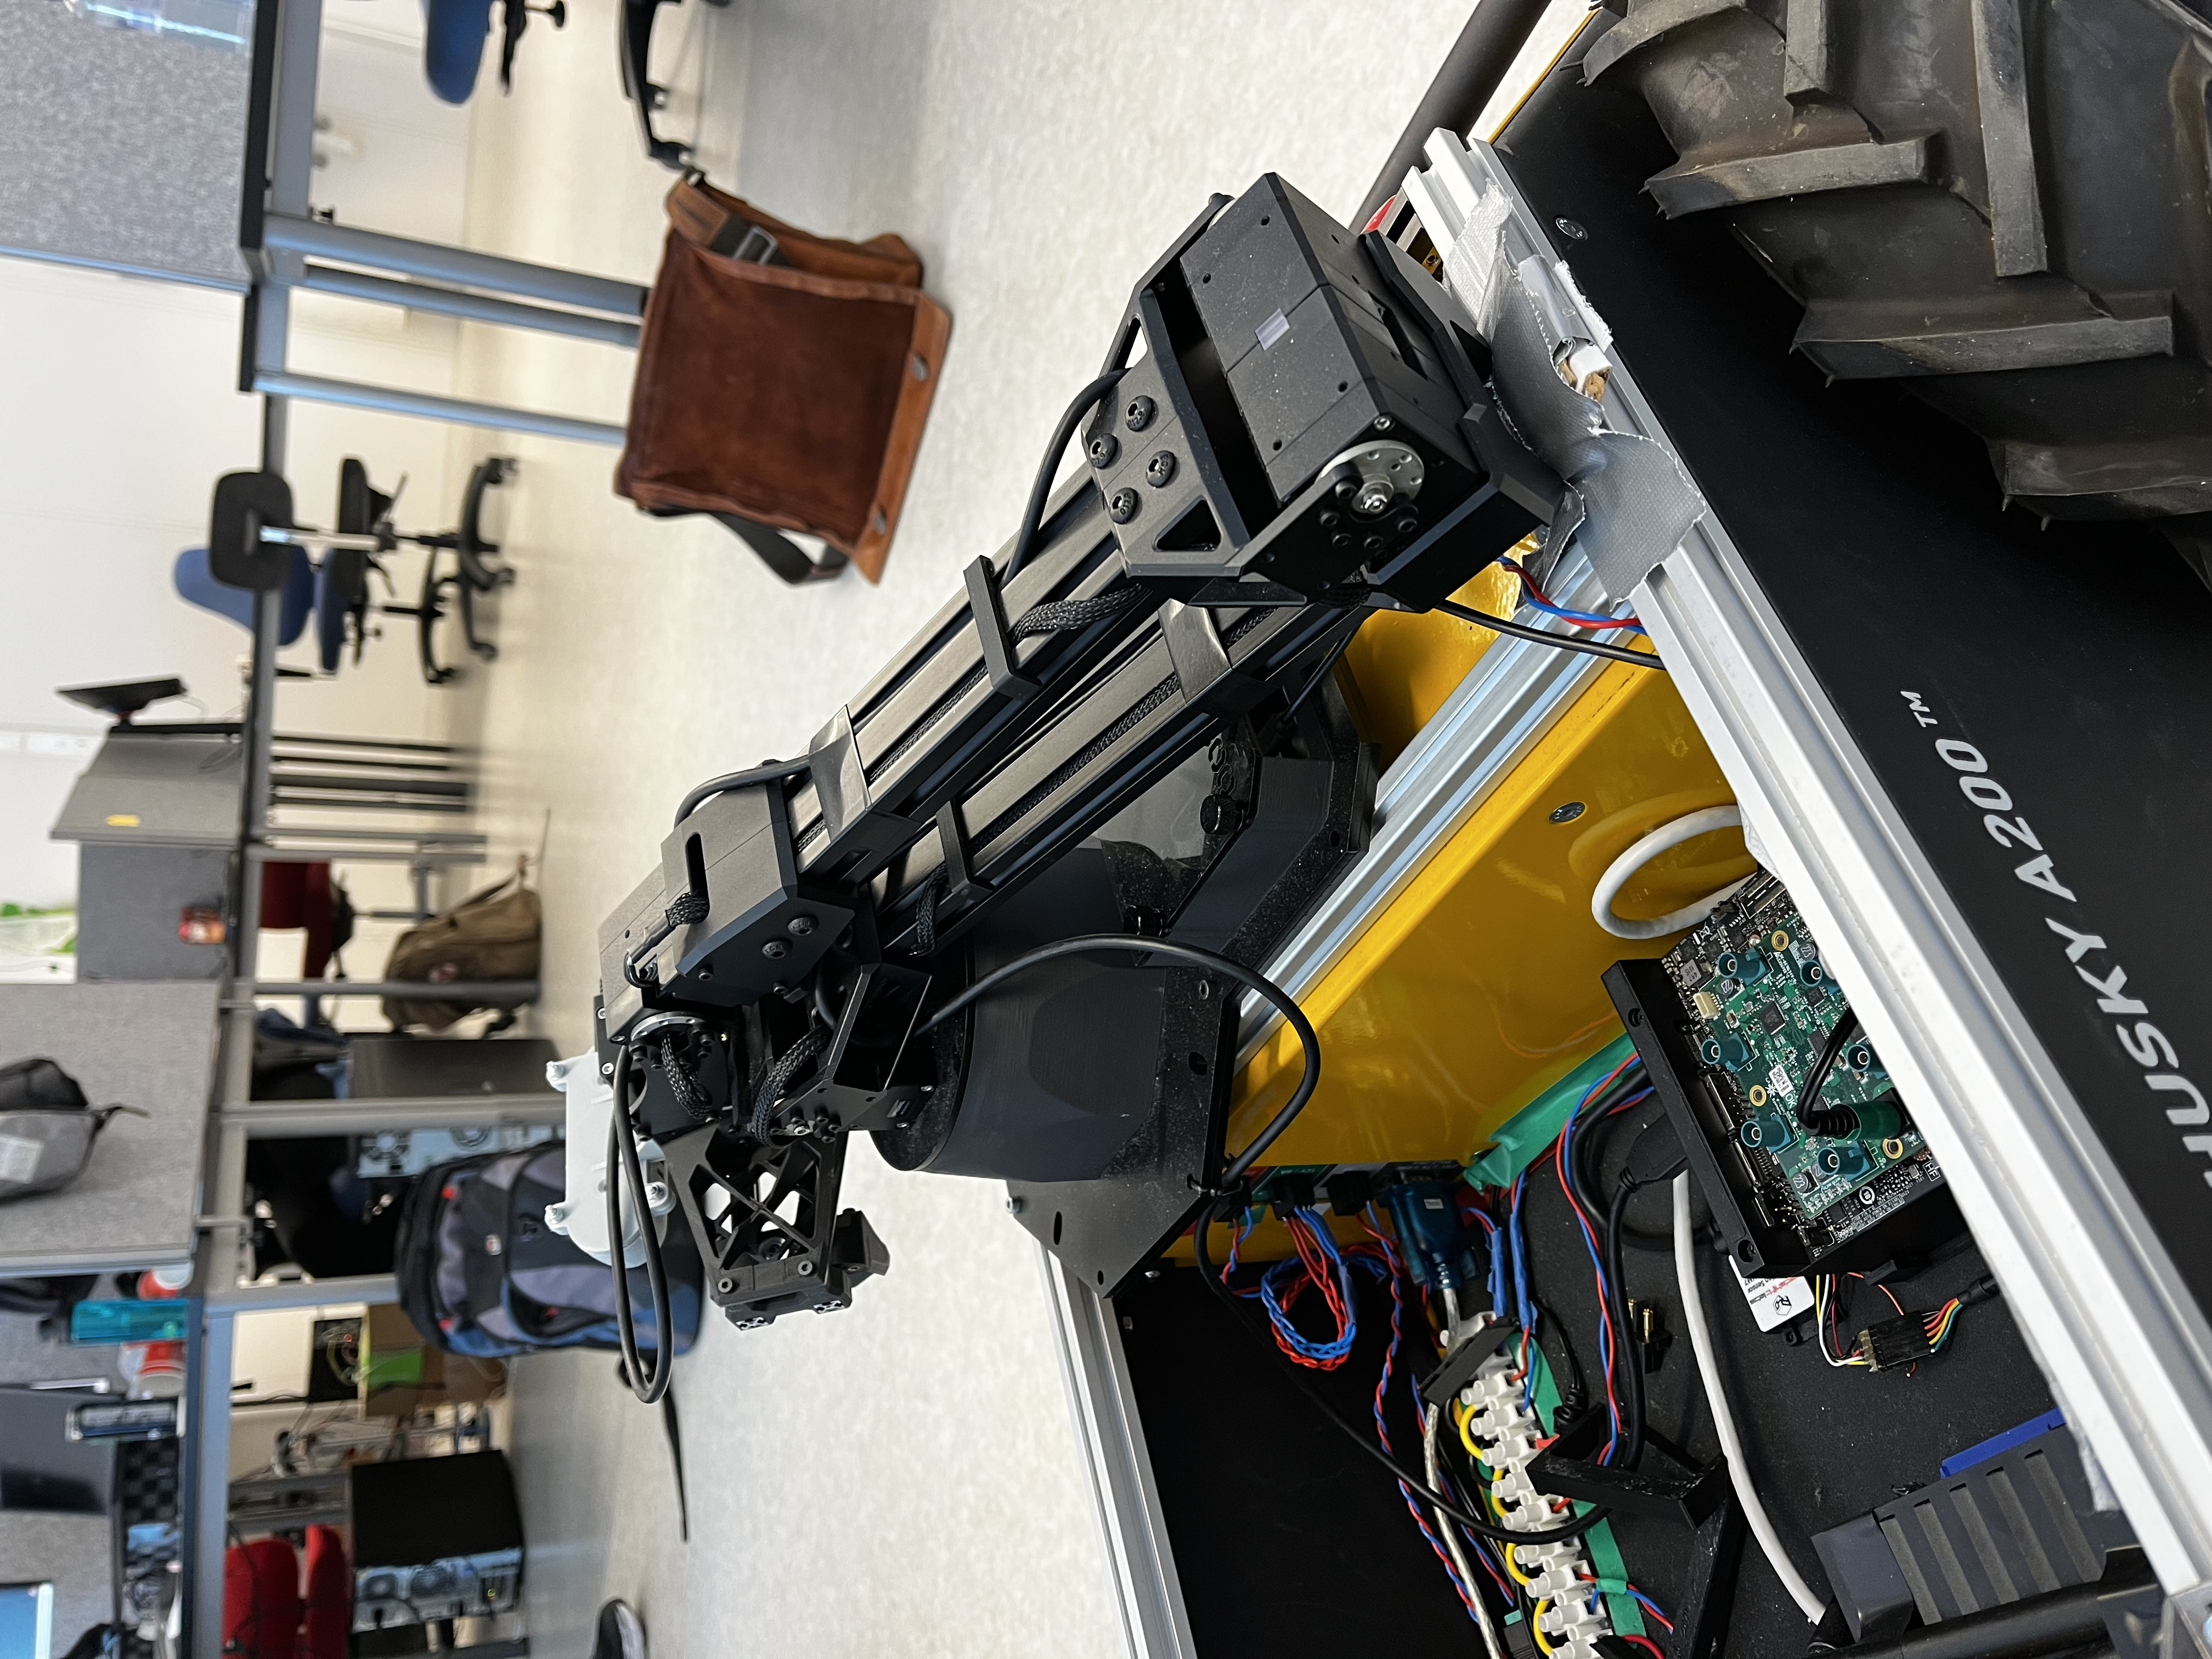
\includegraphics[angle=-90,width = 0.8\textwidth]{Figures/figVX300PhysComplete5.jpg}
  \end{minipage}
  \caption{Interbotix VX300 manipulator mounted on the Husky A200 UGV along with the manipulator mounted Realsense D435i camera. The Manipulator, although powered off in the image, receives it's power through the UGV's 12V power supply and controlled via an on-board Nvidia Jetson AGX Xavier Computer.}
  \label{fig:M:H:M:M:MMC:Vx300Complete}
\end{figure}

% \section{Mobile Robot Configuration}
% For the different components of the robotic system to act together, some software configuration has to be done. This section describes different  parts of the software setup to achieve an autonomously navigating robotic platform. As mentioned in \textbf{HERE, I HAVE TO MENTION A SECTION} ROS2 is used for software implementation. All ROS2 packages described in this section is either available as open source packages, or developed during the course of this project.


\section{Autonomous Navigation}
In order to achieve autonomous navigation of a mobile robot, some requirements first has to be met. The robot needs to be able to estimate its own movement based on the kinematics of the vehicle and the encoder feedback from the wheels. This is done through the motion control system described in section \ref{sec:M:AN:MotionControl}. The UGV needs some form of perception system to help determine its absolute position within the environment. This is done through the perception system described in section \ref{sec:M:AN:Perception}. Lastly has to be a map of the surrounding environment, so that the UGV can place itself somewhere on this map. This map is created with the use of SLAM \ref{sec:M:AN:MappingAndLocalization}. With all these requirements fulfilled, an autonomous navigation system can be put together. The navigation system will take care of both global and local path planning, and send velocity commands to the motion control system based on the calculations. A high level illustration of how the different subsystems interact to achieve autonomous navigation, can be seen in figure \ref{fig:M:AN:ANMethod}.

\begin{figure}[H]
  \centering
  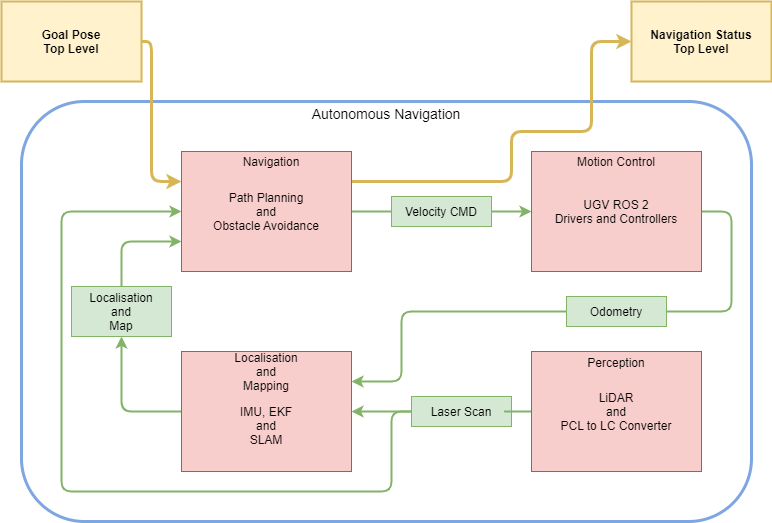
\includegraphics[width = 1\textwidth]{Figures/figANMethod.drawio.png}
  \caption{Overview of autonomous navigation system. Motion Control provides odometry information, which is fused with IMU data in an EKF. The resulting filtered odometry is fed to SLAM along with Laser Scan from a LiDAR. SLAM then provides mapping and localisation for the navigation system. Path planning and collision avoidance is preformed in the navigation system which sends command velocities to the motion control system based on info.}
  \label{fig:M:AN:ANMethod}
\end{figure}

\subsection{Motion Control}\label{sec:M:AN:MotionControl}
The Husky software is put together of several systems that work together in the ROS2 network. Here, the UGV working principle will be described from the nodes that handles input commands to estimated position output that is published to the ROS2 network.

\subsubsection{UGV Setup}
An adaptation of Clearpath's own Husky A200 ROS2 packages are used to operate the UGV in ROS2. Clearpath husky provides Debian ROS2 packages for ROS2 Foxy, and these are therefore used. The story is different for ROS2 Galactic which has reached its EOL and is no longer maintained. Nevertheless, the official Husky ROS2 repository\cite{husky_repo} still contains a branch for ROS2 Galactic even though it won't build. This branch is forked and modified in order to build as well as modified to take in some arguments to the launch file. The forked repository is public and available at \cite{uia_husky_repo}. 

\subsubsection{IMU Setup}
To be able to use the UM7 IMU with ROS2, it has to be set up as a ROS2 node. This is done by using UM7 ROS2 packages provided by \cite{um7_repo}. This node sets a connection to the UM7 IMU through USB and publishes measurements to the ROS topic "/imu/data". The node is dependent on \cite{serial_repo} which is a library for interfacing with serial communication.

\subsubsection{Model Description} \label{sec:M:CS:UGV:S:ModelDescription}
In ROS2, urdf files are used to describe robotic systems. As extra hardware is mounted on the UGV, some extra urdf information has to be added in order to describe the spatial relationship between the UGV and accessories such as the LiDAR. This information is added in an own urdf file and passed upon launch of the husky.

A visual representation of the UGV with all accessories attached is preferable when interacting with the robot in Rviz2. An ope source library for the 3D CAD software Solidworks called "Solidworks to URDF Exporter" \cite{urdf_exporter} is used to export a CAD model of the assembly to urdf. The exporter creates a ROS compatible description package of the CAD model with transforms at user defined locations. The package itself is not used, as it is incompatible with ROS2. However, relevant urdf code and associated ".stl" mesh files is extracted and used when launching the Husky UGV.

\subsubsection{Velocity Commands}
The input velocity commands come from various sources such as a controller or navigation servers. These commands are published at topics to the ROS2 network. As illustrated in figure \ref{fig:rqt_teleop}, these topics are handled through the twist\_mux node. This node publishes velocity commands based on the incoming commands and the defined priority. The command is published to the \\/husky\_velocity\_controller/cmd\_vel\_unstamped topic which is used by the husky velocity controller later to process the incoming commands.

\begin{figure}[H]
  \centering
  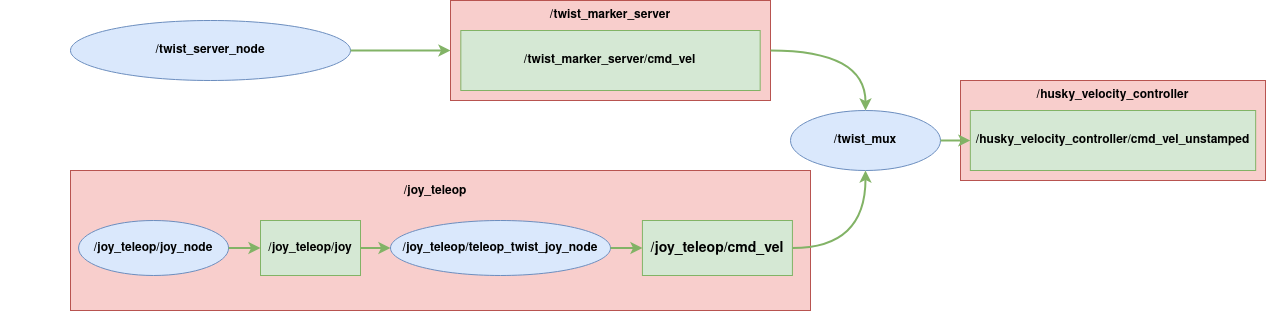
\includegraphics[width = 0.98\textwidth]{Figures/husky_teleop.drawio.png}
  \caption{Example of how velocity commands are handled by twist\_mux node. In this example, it takes in velocity commands from the /joy\_teleop/cmd\_vel topic and the /twist\_marker\_server/cmd\_vel topic. It then forwards the velocity command based on defined priorities to the /husky\_velocity\_controller/cmd\_vel\_unstamped topic.}
  \label{fig:rqt_teleop}
\end{figure}

\subsubsection{Controller}
The velocity command coming from the /twist\_mux server needs to be handled by a controller in order to actuate the UGV. In the ROS2 network, this controller is represented as the husky\_velocity\_controller node. This node takes in velocity commands from the twist\_mux node, actuates the wheel motors and then calculates the motion of the UGV. The resulting odometry is published to the ROS2 topic "/odom".

\subsubsection{Extended Kalman Filter}
In order to more accurately calculate the movement of the UGV, an extended kalman filter is use. The ekf filter fuses UGV odometry with IMU data from both the UM7 IMU and OS1 LiDAR's built in IMU. Figure \ref{fig:rqt_ekf} illustrates how the extended kalman filter(ekf\_node) takes in odometry data from the UGV(husky\_velocity\_controller) as well as IMU data from the UM7 IMU(um7\_driver) and the OS1 LiDAR(ouster\_driver). The node ekf\_node then fuses the odometry and IMU data in order to calculate the transform from /odom to /base\_link.

\begin{figure}[H]
  \centering
  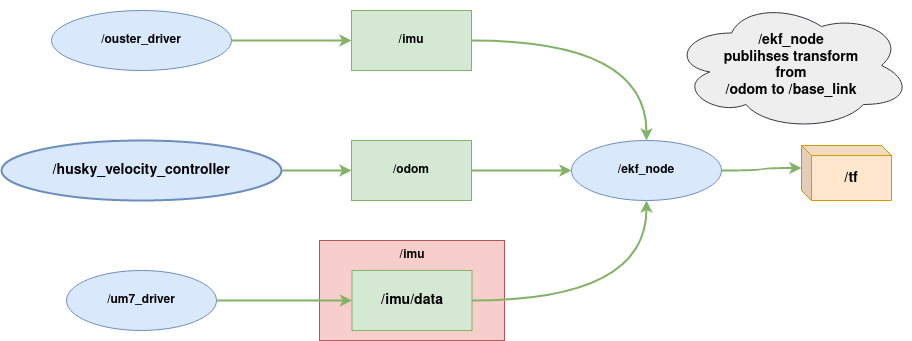
\includegraphics[width = 1\textwidth]{Figures/husky_nodess.drawio.png}
  \caption{Illustration of how the ekf\_node fuses the odometry from the husky\_velocity\_controller and IMU data from both the ouster\_driver and the um7\_driver.}
  \label{fig:rqt_ekf}
\end{figure}

\subsection{Perception}\label{sec:M:AN:Perception}
The perception system of the UGV consists of the Ouster OS1 LiDAR. This LiDAR provides the UGV with 3D spatial information about the environment i the form of a PointCloud. However, the NAV2 navigation stack is made for 2D navigation. That is, the navigation system sets up a 2D birds eye view map of the environment and navigates this map using x, y and yaw coordinates. Therefore, the navigation system requires a 2D map.
In order to build a 2D map of the environment, a measurement structured in 2D is needed. In ROS2, this measurement is presented in the LaserScan data type.

\subsubsection{LiDAR Setup} \label{sec:M:MRC:LiDARSetup}
The Ouster OS1 LiDAR provides a perception aspect to the robotic system that is used to map the surrounding environment. The LiDAR is set up with ROS2 using the ROS2 packages provided by Ouster\cite{ouster_repo}, ros2\_ouster and ouster\_msgs. The package ouster\_msgs contains definitions of data types used by ros2\_ouster. The other package, ros2\_ouster, interfaces the measurements done by the LiDAR with the ROS2 network. This way, the data can be used by other nodes on the ROS2 network.

The LiDAR configurable with a parameter file of the type ".yaml" that can be passed to the ros2\_ouster node upon launch. Table \ref{tab:lidar_params} describes the parameters that are changed and their value compared to the default value.

\begin{table}[H]
\centering
\caption{This table describes the LiDAR parameters that are changed for this project. Their current value and a short description of the parameter as well as their default value.}
\label{tab:lidar_params}
\vspace{1mm}
\begin{tabular}{llll}
\hline
\textbf{Parameter} & \textbf{Value}                                                        & \textbf{Description}                                                                                                           &  \\ \hline
lidar\_ip          & 169.254.171.185                                                       & \begin{tabular}[c]{@{}l@{}}IP address of LiDAR\\ \textbf{Default:} 10.5.5.96\end{tabular}                                               &  \\
computer\_ip       & 192.168.0.169                                                         & \begin{tabular}[c]{@{}l@{}}IP adress of Computer\\ \textbf{Default:} 10.5.5.1\end{tabular}                                              &  \\
sensor\_frame      & lidar\_link                                                           & \begin{tabular}[c]{@{}l@{}}TF2 base frame of sensor\\ \textbf{Default:} laser\_sensor\_frame\end{tabular}                               &  \\
laser\_frame       & base\_laser                                                           & \begin{tabular}[c]{@{}l@{}}TF2 dara frame of sensor\\ \textbf{Default:} laser\_data\_frame\end{tabular}                                 &  \\
timestamp\_mode    & \begin{tabular}[c]{@{}l@{}}TIME\_FROM\\ \_ROS\_RECEPTION\end{tabular} & \begin{tabular}[c]{@{}l@{}}Where the messages timestamp should \\ come from\\ \textbf{Default:} TIME\_FROM\_INTERNAL\_OSC\end{tabular}  &  \\
proc\_mask         & IMG|PCL|IMU                                                           & \begin{tabular}[c]{@{}l@{}}Which data that should be published to \\ the ROS2 network\\ \textbf{Default:} IMG|PCL|IMU|SCAN\end{tabular} &  \\ \hline
\end{tabular}
\end{table}

A parameter change that is worth noticing, is the removal of "SCAN", from the parameter "\textit{proc\_mask}. This removes the LaserScan output from the LiDAR. The reason for this is that the conversion from PointCloud to LaserScan is done by another ROS2 Node. This is further explain in section \ref{sec:M:AN:Perception}.

\subsubsection{PointCloud to LaserScan} \label{sec:M:AN:P:PointCloudToLaserScan}
As mentioned earlier in section\ref{sec:M:MRC:LiDARSetup}, the LaserScan output from the Ouster OS2 LiDAR is removed. The LaserScan published by \lstinline{ros2_ouster} use the measurement from the laser that is physically oriented closest to horizontal in the LiDAR. This creates a LaserScan that measures a horizontal 2D plane around the sensor, which is how 2D $360\deg$ LiDARs usually work. However, the Husky A200 combined with all its accessories is a tall robot and having information of how a 2D plane in the environment around it looks is insufficient. Additionally, it's LiDAR provides 3D information of the environment. Therefore, the ROS2 package \lstinline{pointcloud_to_laserscan} takes care of the conversion from PointCloud to LaserScan. This gives the possibility to define a minimum and maximum height that should be converted to LaserScan. For example, the developer could say that all points from 0.1[m] above ground to 0.1[m] above the highest point of the UGV should be considered when creating the LaserScan signal. This method takes advantage of the 3D PointCloud data set when creating a LaserScan of the surrounding area. The Resulting 2D map will therefore be valid for the whole UGV and not only for the plane where the LiDAR is located.


\subsection{Mapping and Localisation} \label{sec:M:AN:MappingAndLocalization}
 Since SLAM algorithms does both mapping and localisation simultaneously, it gives an accurate representation of an environment for navigation. In this project, the ROS2 package slam\_toolbox is used to run an online asynchronous SLAM node for mapping. This ROS2 node takes in odometry information from the motion control system together with LaserScan from the perception system to localise and generate a 2D map of the environment. Because of the use of "PointCloud to LaserScan", the resulting algorithm maps all obstacles in the "collision zone" of the UGV to the map. Obstacles that are too low to be mapped can be traversed by the UGV. Obstacles that are located so high that the UGV could go under it, won't be mapped. When looking at localisation, there are several methods that could be used. As SLAM is already used for mapping, it becomes a natural choice for preforming the localisation task as well. SLAM Toolbox utilises a pose-graph approach to the localisation and mapping problem. This is similar to the one described in section \ref{sec:T:AN:L:SLAM}.

\subsection{Navigation}
As the UGV platform is set up with compatible motion control, perception, mapping and localisation systems, it is able to run the ROS2 Navigation stack NAV2. 

\textbf{DESCRIBE NAV2 FURTHER! I DOESNT GIDD NOW - ØØ 24.04}


\section{Pick and Place} \label{M:PickAndPlace}
\textbf{WRITE ABOUT PICK AND PLACE TASK OR MOVE FROM EARLIER}

\begin{figure}[H]
  \centering
  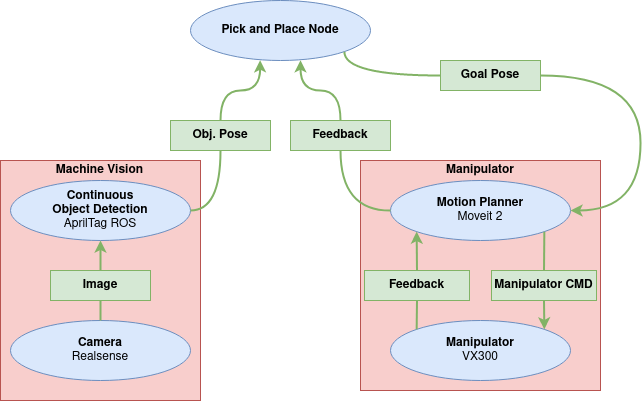
\includegraphics[width = 1\textwidth]{Figures/figPickAndPlaceMethod.drawio.png}
  \caption{This figure illustrates the Pick and Place subsystem}
  \label{fig:M:PAP:PickAndPlaceMethod}
\end{figure}

\subsection{Manipulator Configuration}\label{sec:M:MRC:Manipulator}
Interbotix provides ROS2 packages for the VX300 manipulator. The most relevant of these being the package \lstinline{interbotix_xsarm_moveit}, which is used to bring up the VX300 manipulator in Moveit2 for motion planning and control of the arm as well as Rviz2 with a GUI for running and testing the Moveit2 configuration. Figure \ref{fig:VX300Moveit} illustrates a virtual VX300 manipulator running with moveit2 and visualised in Rviz2. The Moveit2 Motion Planning GUI is located in the lower left corner of the figure. The actual manipulator pose is illustrated by a black manipulator and the goal pose is illustrated by an orange manipulator. In figure \ref{fig:VX300Moveit}, the manipulator is oriented at the goal pose. The orange goal pose shines through the actual pose at the fingers.

\begin{figure}[H]
  \centering
  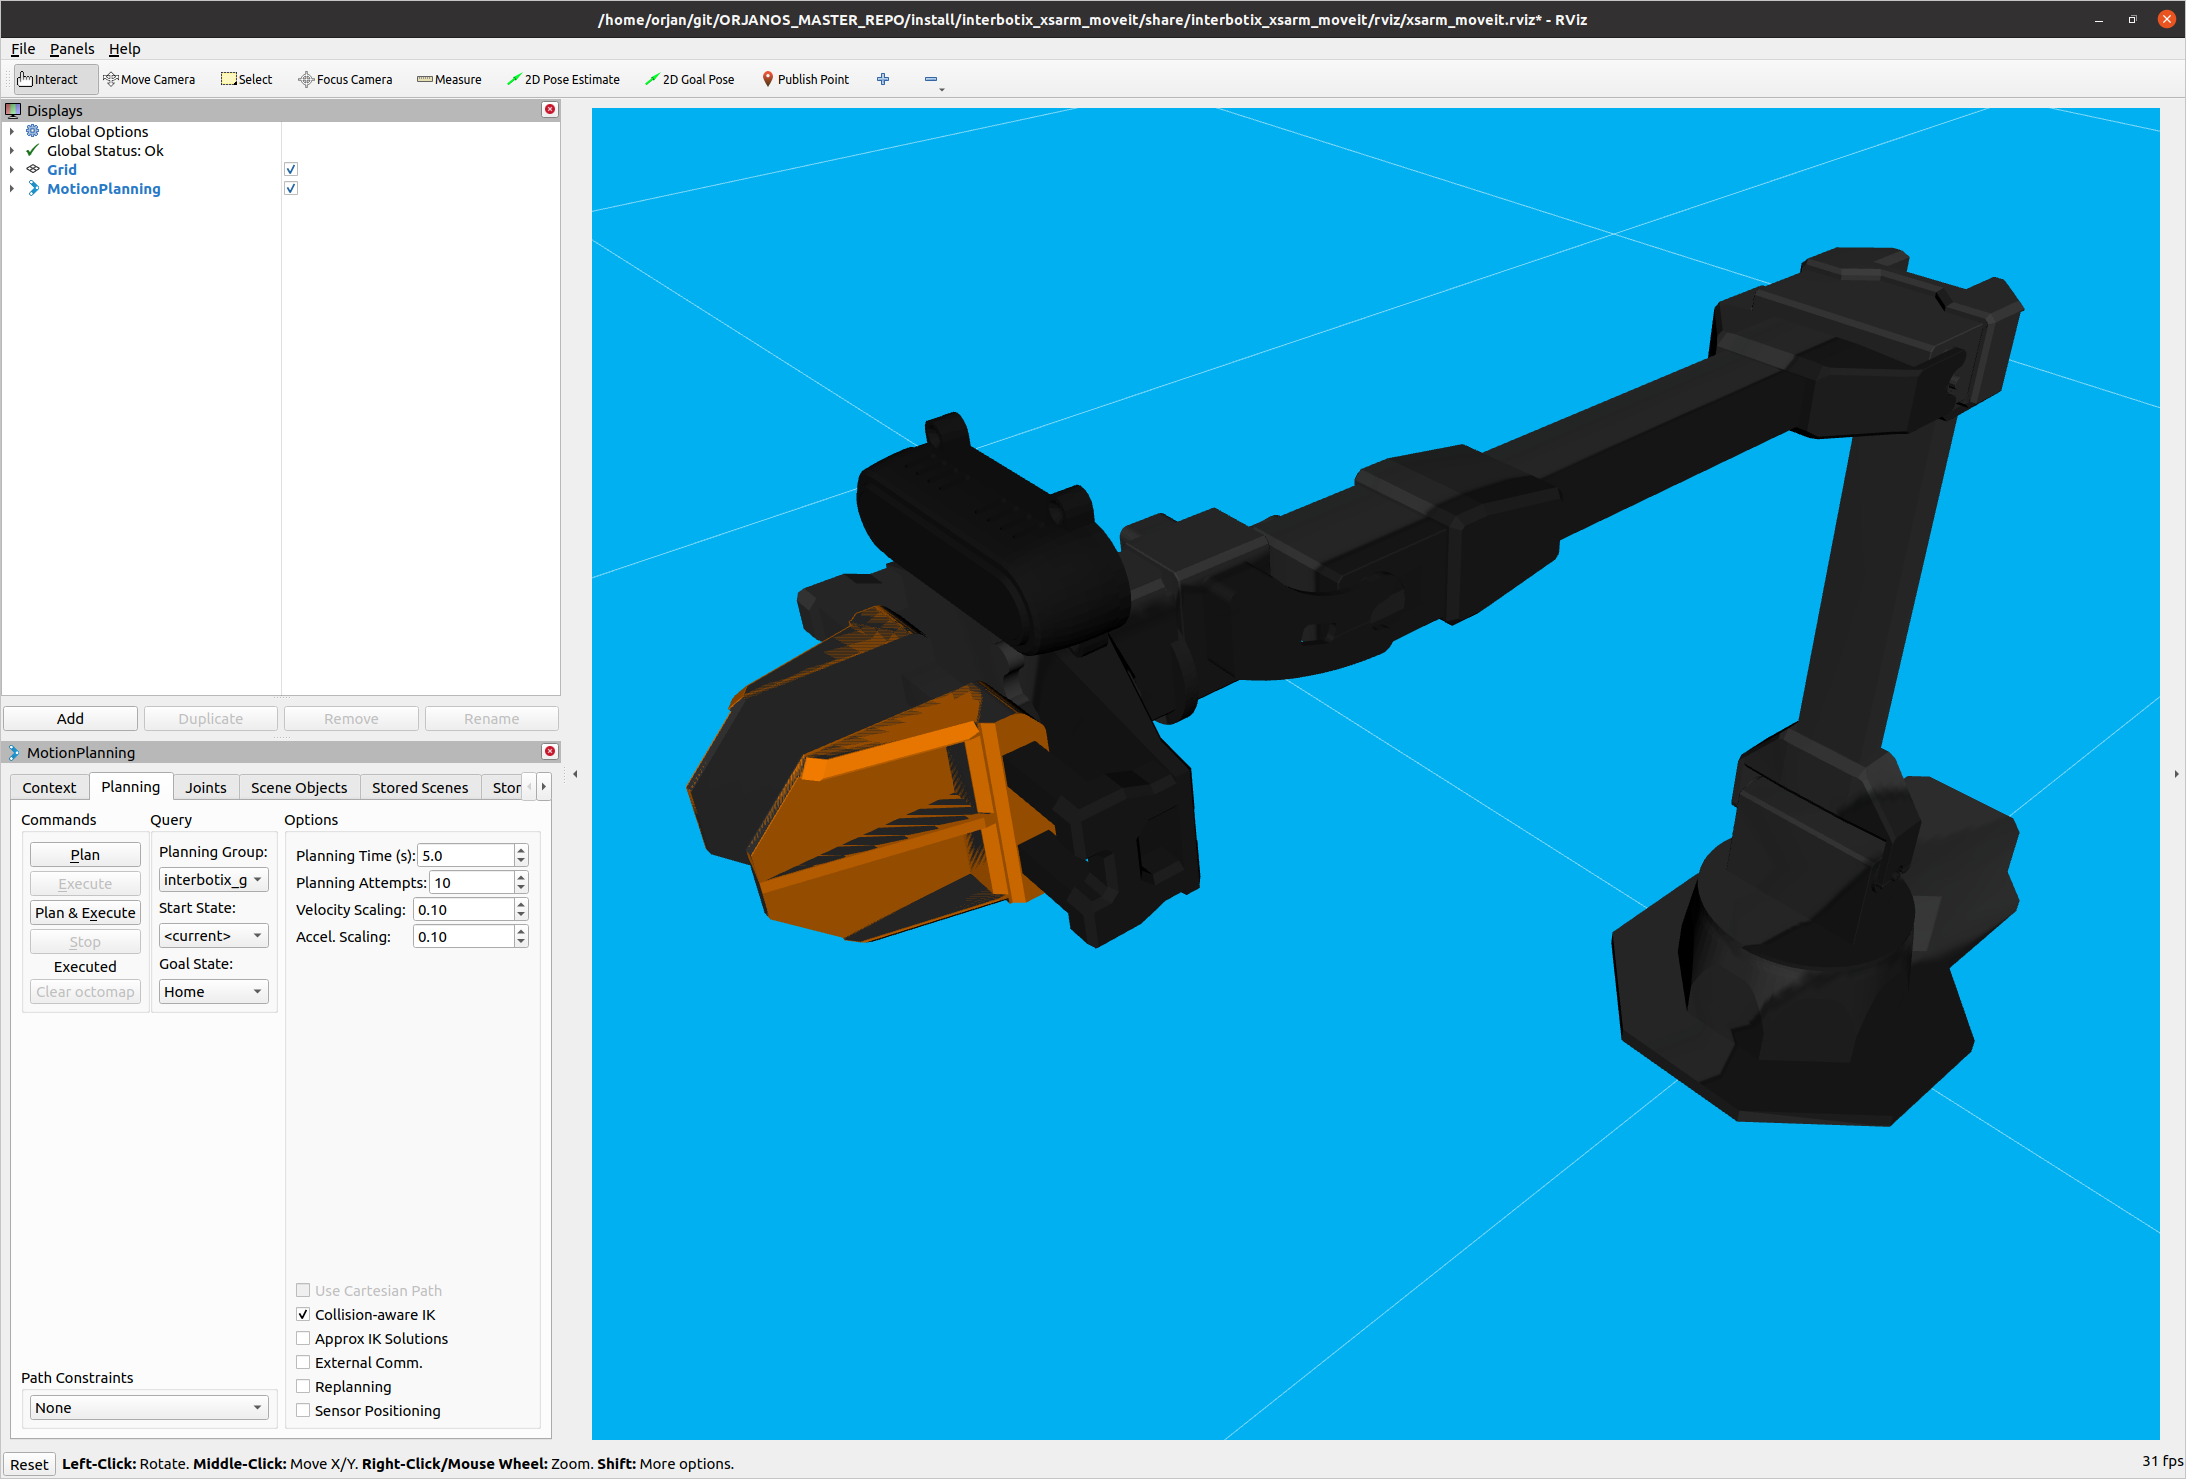
\includegraphics[width = 1\textwidth]{Figures/figVX300Moveit.png}
  \caption{A virtual VX300 manipulator running moveit2 and visualised in Rviz2. The Moveit2 Motion Planning GUI is located in the lower left corner of the figure. The actual manipulator pose is illustrated by a black manipulator and the goal pose is illustrated by an orange manipulator which shines through at the gripper fingers. The Realsense camera can be seen mounted on top of the gripper.}
  \label{fig:VX300Moveit}
\end{figure}

\subsubsection{Model Description}
Looking at figure \ref{fig:VX300Moveit}, it can be seen that the Realsense camera, described in section \ref{sec:M:CS:UGV:S:ModelDescription}, is mounted on top of the VX300 gripper using its mounting bracket. This is practical for visualisation, but also necessary to avoid collisions with both surrounding objects, and the manipulator itself. Similarly to how accessories were added to the UGV in section \ref{sec:M:CS:UGV:S:ModelDescription}, the Realsense camera assembly is generated through the open source urdf exporter\cite{urdf_exporter}. 

\subsubsection{Planning Scene}
In Moveit2, the planning scene describes the environment where the manipulator is located. Objects and barriers described in the planning scene will be taken into account by the planner when planning a manipulator motion. As this manipulator is mounted on top of the UGV, the manipulator needs to have a perspective of the shape and position of the UGV in order to avoid collision. As mentioned in section \ref{sec:M:CD:InitialConcept}, the UGV is running on the "UGV Xavier", and the manipulator is running on the "Manipulator Xavier". Both these robotic devices are described by xacro files on the form of urdf. However, they take in pure urdf files for accessories. This means that it is no easy way to add the urdf file of one as an accessory to the other. As a result, the robotic description of the UGV and the manipulator is separated. To take the UGV into account when planning manipulator motion, the shape of the husky is therefore added to the planning scene in Moveit2 as collision boxes.

In the Motion planning GUI seen in the lower left corner of figure \ref{fig:VX300Moveit}, collision boxed can be added to the planning scene through the "Scene Objects" tab. This is a simple interface where it is possible to add different geometric shapes with a defined size and position. After defining a planning scene, the scene can be exported to a ".scene" file which can be used later to import the same scene. In this project, a ROS2 node that parses ".scene" files and publishes the information in them to the manipulator's planning scene is developed. This node is described more thoroughly later in section \ref{sec:M:A:SceneGeometryPublisher}.

\subsection{Machine Vision} \label{sec:M:MRC:MachineVision}
The machine vision system is comprised by an Intel Realsense D435i, as described in section \ref{sec:M:H:P&PH:ManipulatorMountedCamera}, and an AprilTag based 6-DOF pose estimation system.

\subsubsection{Vision Camera} 
The gripper mounted Realsense camera is used for the machine vision system during this project. Intel provides ROS2 packages for Realsense cameras that interfaces with the ROS2 network \cite{realsense_ros_repo}. These packages publishes the data from the Realsense camera to the ROS2 network so that it is available for other nodes on the network. The ROS2 Realsense packages requires Intel RealSense SDK 2.0 which is available as debian packages for AMD Ubuntu machines. For Xaviers, whom are running an ARM architecture, the SDK is available to be built from source on Github\cite{realsense_jetson_guide}.

\subsubsection{Tag Detection System} \label{sec:M:MRC:MV:TagDetectionSystem}
Together with the Realsense camera, an AprilTag detection system is set up using the open source packages provided by \cite{apriltag_repo}, \cite{apriltag_ros_repo} and \cite{apriltag_msgs_repo}. These packages are used to create a ROS2 node that will run continuous AprilTag detection on the defined camera stream. AprilTag is, as described in section \ref{sec:T:OD:TagBasedObjectDetection} a tag based system for 6-DOF pose estimation using a monocular vision system. Section \ref{sec:T:OD:TagBasedObjectDetection} also mentions tag families, that are collections of pre-defined AprilTags for use by developers. In this project, the standard tag family "\textit{tag36h11}" is used. The AprilTag ROS2 node requires tags to be defined in a \textit{".yaml"} file. An example of a tag definition can be seen in listing \ref{lst:M:M:MachineVision}.

\begin{lstlisting}[language=XML, label=lst:M:M:MachineVision, caption={Example of AprilTag tag definitions in a ".yaml" file. This example defines two tags of different names, using the tag id 0 and 1 in the defined tag family The size is alse defined for each tag. The tag family (tag36h11) is set in another parameter file.}]
/**:
  ros__parameters:
    standalone_tags:
      tag_names: ["my_tag_0", "my_tag_1"]
      my_tag_0:
        id: 0
        size: 0.135
      my_tag_1:
        id: 1
        size: 0.0344
\end{lstlisting}

In listing \ref{lst:M:M:MachineVision}, the tags "my\_tag\_0" and "my\_tag\_1" are defined. The "id" parameter on each tag definition links this definition to a specific AprilTag in the AprilTag family \textit{"tag36h11"}. This way, when the AprilTag detection node detects an AprilTag in the camera stream, it will check if the detected tag is defined in the tag definition "\textit{.yaml}" file. If so, it will use the defined size and location in the camera stream to publish a 6-DOF pose of the tag to the ROS2 network. The published pose will be on the form of a TF2 transform with the same name as the tag (ex. "my\_tag\_0").

\subsection{Scene Geometry Publisher} \label{sec:M:A:SceneGeometryPublisher}
As mentioned when describing the planning scene in section \ref{sec:M:MRC:Manipulator}, a ROS2 node that parses a "\textit{.scene}" file and publishes the information in this file to the planning scene. This node consists of a custom C++ Class, the implementation of this class, a launch file and a "scene" folder to put \textit{.scene} files. An UML class representation of the ScenePublisher class can be seen in figure \ref{fig:scenePublisherUML}. It appears alone in the UML Class diagram as the interactions between other nodes happens through the ROS2 network.

\begin{figure}[H]
  \centering
  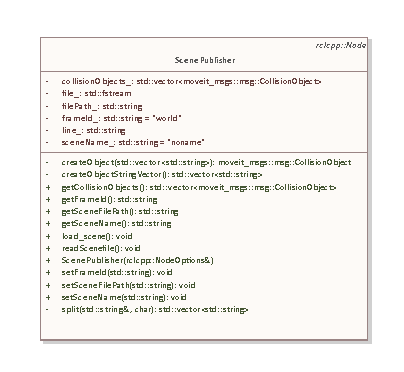
\includegraphics[width = 0.8\textwidth]{Figures/scene_geometry_publisher.pdf}
  \caption{UML Class Diagram of the Scene Geometry publisher Node. As this is one class and interacts through ROS topics, it appears alone in the class diagram.}
  \label{fig:scenePublisherUML}
\end{figure}

It can be seen from figure \ref{fig:scenePublisherUML} that ScenePublisher inherits from "rclcpp::Node". This means that ScenePublisher will have all the functionality of a standard C++ node in addition to the functionality added to it. When an instance of a ScenePublisher is initiated, it will run the constructor (\lstinline{ScenePublisher(rclcpp::NodeOptions&)}, which sets the scene file path to the default path (.scene file in scene folder of the package). The constructor requires an \lstinline{rclcpp::NodeOptions}variable where the developer is able to pass custom node options to the node. 

Upon initiation of a ScenePublisher node, the \textit{.scene} file path ca be changed using the \lstinline{setSceneFilePath()} method. Furthermore, \lstinline{readSceneFile()} should be used to read the specified \textit{.scene} file and store the information in the member variables of the class. After this, the method \lstinline{loadScene()} can be used to publish the collision objects specified by the .scene file. The private methods \lstinline{createObject()} and \lstinline{createObjectString()} is used by other methods in the class to create a collision object of the correct data type. The class also contains a private \lstinline{split()} method that splits up a string based on the defined input char. Other than that, there are methods to set and get the values of different member variables.

An example implementation of this package is shown in appendix \ref{A:lst:ScenePublisher} this implementation first publishes static collision objects to the scene, before applying collision objects to the manipulator from another "\textit{.scene}" file. 

% It can also be seen that \lstinline{frameID_} is hard coded to "\textit{world}", the default base link of Interbotix manipulators.

\subsection{Husky Pick and Place Package} \label{sec:M:A:HuskyPickAndPlace}
In order to easier interact with Moveit2, a custom "Pick and Place" node is developed. This node listens for incoming commands through the custom ROS2 topic "\textit{/action}" and provides feedback about its operating status on the custom ROS2 topic "\textit{/action\_status}". Based on the incoming commands, the node will preform different pick and place related operations with the Interbotix VX300 manipulator. The node consists of a C++ class and the implementation of this class. As with the scene publisher, an UML class diagram of the C++ class is made. The diagram can be seen in figure \ref{fig:PickAndPlaceUML}.

\begin{figure}[H]
  \centering
  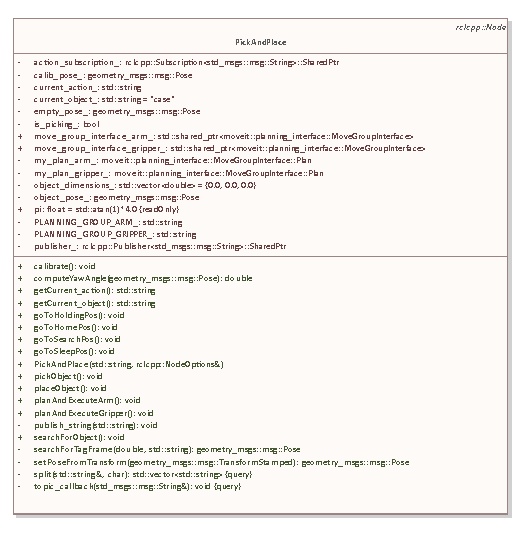
\includegraphics[width = 0.8\textwidth]{Figures/husky_pick_and_place.pdf}
  \caption{UML Class Diagram of the Husky Pick and Place Node. As this is one class and interacts through ROS topics, it appears alone in the class diagram.}
  \label{fig:PickAndPlaceUML}
\end{figure}

The robotic manipulator is limited to 5 degrees of freedom. This restricts the manipulators ability to reach certain positions. Therefore, the target poses has to take this into account. This problem is most prevalent when picking, as the target object could have any pose.
The chosen solution is to always pick the target objects from the top. This solution places a restriction on the object in that it has to be placed on a level surface. The x-rot and y-rot of the object has to be assumed to be level with the manipulator base. Then, only xyz-position and z-rot  will be taken into account when picking the object.




\section{Top Level} \label{M:TopLevel}
% During the course of this thesis, a few custom ROS2 packages were made from scratch. These are ROS2 packages made to suit a need at a specific point of the thesis. For instance, "Scene Geometry Publisher" (section \ref{sec:M:A:SceneGeometryPublisher}) is used to parse a ".scene" file and publish objects to the Moveit2 planning scene. While, "Husky Pick and Place" (section \ref{sec:M:A:HuskyPickAndPlace}) waits for a command on a custom ROS2 topic before preforming pick and place related manipulator operations. Lastly "Husky Master" (section \ref{sec:M:A:HuskyMasterNode}) is the node that interacts with NAV2 and "Husky Pick and Place" and orchestrates these nodes in order to achieve autonomous warehouse product fetching.

%\subsection{Husky Master Node} \label{sec:M:A:HuskyMasterNode}

On a high level, the system is controlled by a top level ROS node, the Husky Master Node, as described in section \ref{sec:M:ConceptualDesign}. 

\subsection{Husky Master Node}
An UML class diagram of the Husky Master Node can be seen in figure \ref{fig:M:TL:huskyMasterUML}.

\begin{figure}[H]
  \centering
  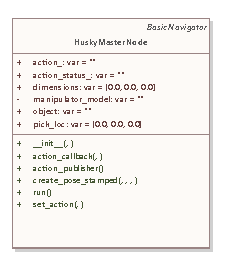
\includegraphics[width = 0.6\textwidth]{Figures/husky_master.pdf}
  \caption{UML Class Diagram of the Husky Master Node. As this is one class and interacts through ROS topics, it appears alone in the class diagram.}
  \label{fig:M:TL:huskyMasterUML}
\end{figure}

% \begin{figure}[htp]
%   \centering
%   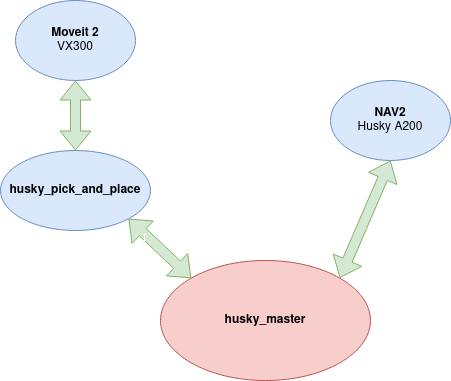
\includegraphics[width = 0.6\textwidth]{Figures/software_overview.drawio.png}
%   \caption{The "husky\_master" node controls the operation by interfacing directly with NAV2 and with Moveit2 through the "husky\_pick\_and\_place" node.}
%   \label{fig:husky_master}
% \end{figure}
